\ifthenelse{\equal{\PRINTABLE}{false}}{
\chapter{Distributions de contrôle -- $\Higgs\to\tau\tau$}\label{annexe-control_plots-HTT}

Cette annexe présente des distributions de contrôle
avant ajustement des paramètres de nuisance
sur les événements utilisés dans l'analyse des événements $\Higgs\to\tau\tau$
présentée dans le chapitre~\refChHTT.
La sélection est \og inclusive \fg, les événements sont ceux sélectionnés par la définition de la région de signal,
sans coupure sur $\mT^{\ell}$ (canaux \mu\tauh, \ele\tauh) ni $\Dzeta$ (canal \ele\mu).
\par
Pour chacune des trois années de prise de données (2016, 2017, 2018)
et
chacun des quatre canaux (\tauh\tauh, \mu\tauh, \ele\tauh, \ele\mu),
les distributions de plusieurs variables sont données.
\par
Dans chacun des graphiques,
les données observées (points noirs) sont comparées à la modélisation des bruits de fond (histogrammes remplis en couleur et empilés).
Les bandes grisées correspondent à l'incertitude statistique totale sur le bruit de fond.
Le rapport au bruit de fond est donné dans la partie inférieure des graphiques.

\bigskip
\par
Ces distributions montrent un bon accord entre données observées et estimations des bruits de fond,
à l'exception:
\begin{itemize}
\item des pseudo-rapidités des \tauh, $\eta(\tauh)$;
%\item de la quantité de jets issus de quarks~\quarkb;
\item du nombre de vertex d'empilement \Npu.
\end{itemize}
%Les membres du groupe de l'analyse MSSM \HAtoTauTau\ 
%ont récemment été mis au courant des écarts observés
%et de plus amples investigations ont été menées.
%Ci-après, les pistes envisagées sont présentées.
\begin{wrapfigure}{R}{.5\textwidth}
\centering
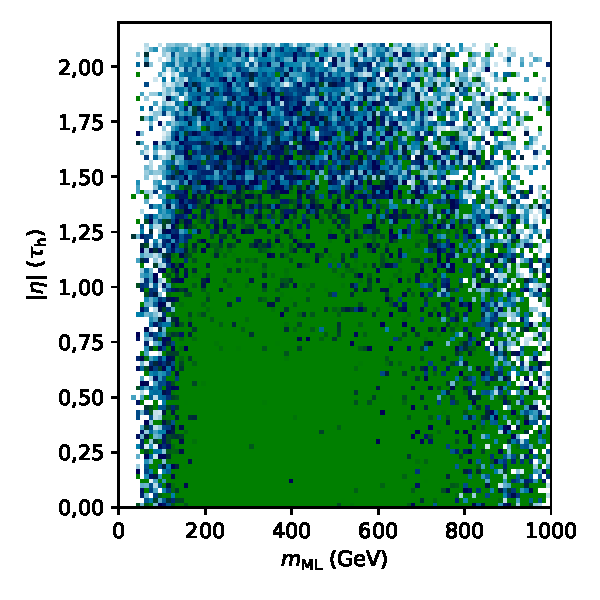
\includegraphics[width=.45\textwidth]{\PhDthesisdir/plots_and_images/my_plots/ML/from_ML_plots/correlations_studies/2D_histo-predictions-leading_tau_eta_reco.pdf}
\caption[Distribution de $\abs{\eta}(\tauh)$ en fonction de \mml.]{Distribution de $\abs{\eta}(\tauh)$ en fonction de \mml.}
\label{fig-2D_histo-predictions-leading_tau_eta_reco}
\end{wrapfigure}
\paragraph{Pseudo-rapidités des \tauh}
L'écart observé pourrait être réduit
en utilisant des \fakefactors\ dépendants de $\eta(\tauh)$,
ce qui n'est pas le cas actuellement.
D'autres variables dépendant directement de la pseudo-rapidité d'un \tauh\ telles que
la distance $\Delta R$ entre les deux éléments du dilepton
montrent également des écarts entre
données observées et estimation des bruits de fond,
potentiellement dus à ceux sur $\eta(\tauh)$.
\par
L'écart sur $\eta(\tauh)$ pourrait avoir un effet sur \mTtot,
cette dernière étant fonction d'impulsions transverses et d'angles azimutaux,
car la projection des impulsions dans le plan transverse,
\begin{equation}
\pT = \frac{p}{\cosh \eta}
\mend[,]
\end{equation}
fait intervenir $\eta(\tauh)$.
Cependant, les modélisations des impulsions transverses et des angles azimutaux sont satisfaisantes.
Les valeurs de \mTtot\ ne sont donc pas affectées par la mauvaise modélisation de $\eta(\tauh)$.
\par
Le réseau de neurones B" utilisé afin d'obtenir \mml, présenté au chapitre~\refChML, exploite les valeurs de $\eta(\tauh)$.
La figure~\ref{fig-2D_histo-predictions-leading_tau_eta_reco} montre la distribution de $\abs{\eta}(\tauh)$ en fonction de \mml.
Bien que les hautes valeurs de $\abs{\eta}(\tauh)$ soient moins représentées à haute \mml,
ce qui peut s'expliquer par l'effet de la projection mentionnée précédemment,
aucune corrélation n'apparaît entre $\abs{\eta}(\tauh)$ et \mml.
Les valeurs de \mml\ ne semblent donc pas affectées par la mauvaise modélisation de $\eta(\tauh)$.
\paragraph{Nombre de vertex d'empilement}
%Les distributions de \Npu\
%montrent un mauvais accord entre données observées et estimations des bruits de fond.
L'effet de la mauvaise modélisation de \Npu\ constatée dans les distributions de contrôle
devrait être marginal sur \mTtot,
car cette observable ne dépend pas de \Npu.
Les autres sources d'incertitudes sur \mTtot\ permettent alors de couvrir cet effet.
\par
Les valeurs de \mml, \ie\ des prédictions du réseau de neurones présenté au chapitre~\refChML,
dépendent de \Npu.
Les bons accords
entre observations et estimations des bruits de fond
obtenus sur les distributions de \mml\
montrent que cette observable semble peu affectée par la mauvaise modélisation de \Npu.
%\par
La figure~\ref{fig-PU_vars_effect} confirme cette hypothèse.
Elle représente l'évolution de la réponse du réseau de neurones,
à basse, moyenne et haute masse ainsi que sur toute la gamme de masse, ces ensembles étant définis au chapitre~\refChML,
lorsque les valeurs de \Npu\ sont modifiées selon
\begin{equation}
\Npu \to \Npu + \Delta\Npu
\end{equation}
avec $\Delta\Npu$ compris entre $-5$ et $+5$.
Les modifications induites sur la réponse du réseau de neurones sont inférieures à \SI{1}{\%} alors que sa résolution relative est de l'ordre de \SI{20}{\%}.
\begin{figure}[h]
\centering
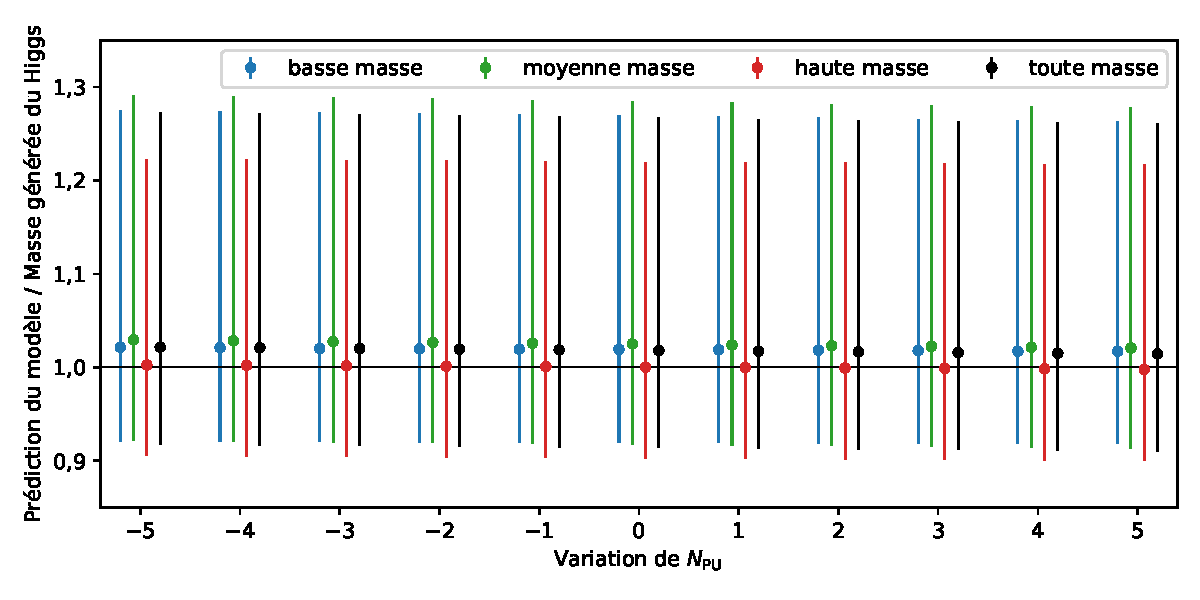
\includegraphics[width=.9\textwidth]{\PhDthesisdir/plots_and_images/my_plots/ML/from_ML_plots/correlations_studies/PU_vars_effect.pdf}
\caption[Variations de la réponse du réseau de neurones en fonction de $\Delta\Npu$.]{Variations de la réponse du réseau de neurones en fonction de $\Delta\Npu$ à basse, moyenne et haute masse ainsi que sur toute la gamme de masse. La résolution à $\pm1\sigma$ est renseignée par les barres verticales.}
\label{fig-PU_vars_effect}
\end{figure}
\par
Ainsi,
l'effet limité de \Npu\ sur les variables discriminantes utilisées
permet de conserver des résultats finaux pertinents
bien que l'écart sur \Npu\
entre observations et estimations des bruits de fond
puisse être de l'ordre de \SI{40}{\%}.
Plusieurs effets peuvent causer cet écart sur \Npu:
\subparagraph{Modélisation des \HLTpaths\ dans les données encapsulées}
Les données encapsulées,
introduites dans le chapitre~\refChHTT,
sont des hybrides entre données réelles et simulées.
Les \HLTpaths\ activés proviennent de la partie simulée uniquement,
\ie\ d'un événement vide à l'exception des leptons~\tau\ qui remplacent les muons.
Or, l'empilement provient de la partie réelle des données encapsulées
et l'acceptation des \HLTpaths\ en dépend.
Actuellement,
des facteurs correctifs sont appliqués en fonction des propriétés cinématiques des \tau\
mais ils ne dépendent pas de \Npu.
Ainsi, les distributions de \Npu\ peuvent être biaisées dans les données encapsulées.
\subparagraph{Dépendance en \Npu\ de l'identification des \tauh}
L'identification d'un \tauh\ dépend de son isolation,
elle-même sensible à l'empilement.
Différents points de fonctionnement
d'identification des \tauh\ sont utilisés dans le cadre des \fakefactors,
introduits au chapitre~\refChHTT.
Ces derniers ne sont pas déterminés en fonction de \Npu,
ce qui peut introduire un biais.
\subparagraph{Modélisation de \Npu\ dans les données simulées}
Un désaccord sur \Npu\ est bien attendu entre données réelles et simulées
et ces dernières sont pondérées afin de le corriger, comme exposé au chapitre~\refChLHCCMS.
Toutefois, cette pondération ne permet pas d'obtenir un accord parfait.

\def\EMBFFchoice{emb_ff}
\def\lolcalcurrentyear{2016}
\def\lolcalcurrentchannel{tt}
\ifthenelse{\equal{\lolcalcurrentchannel}{tt}}{\def\localchannel{\tauh\tauh}\def\localLA{\ensuremath{\tauh^{(1)}}}\def\localLB{\ensuremath{\tauh^{(2)}}}}{}
\ifthenelse{\equal{\lolcalcurrentchannel}{mt}}{\def\localchannel{\mu\tauh}\def\localLA{\mu}\def\localLB{\ensuremath{\tauh}}}{}
\ifthenelse{\equal{\lolcalcurrentchannel}{et}}{\def\localchannel{\ele\tauh}\def\localLA{\ele}\def\localLB{\ensuremath{\tauh}}}{}
\ifthenelse{\equal{\lolcalcurrentchannel}{em}}{\def\localchannel{\ele\mu}\def\localLA{\ele}\def\localLB{\mu}}{}

\begin{figure}[p]
\centering

\subcaptionbox{Impulsion transverse du jet principal.}[.475\textwidth]
{\plotHTTcontrol{\lolcalcurrentyear}{\EMBFFchoice}{\lolcalcurrentchannel}{jpt_1}\vspace{-.125\baselineskip}}
\hfill
\subcaptionbox{Impulsion transverse du jet secondaire.}[.475\textwidth]
{\plotHTTcontrol{\lolcalcurrentyear}{\EMBFFchoice}{\lolcalcurrentchannel}{jpt_2}\vspace{-.125\baselineskip}}

\subcaptionbox{Pseudo-rapidité du jet principal.}[.475\textwidth]
{\plotHTTcontrol{\lolcalcurrentyear}{\EMBFFchoice}{\lolcalcurrentchannel}{jeta_1}\vspace{-.125\baselineskip}}
\hfill
\subcaptionbox{Pseudo-rapidité du jet secondaire.}[.475\textwidth]
{\plotHTTcontrol{\lolcalcurrentyear}{\EMBFFchoice}{\lolcalcurrentchannel}{jeta_2}\vspace{-.125\baselineskip}}

\subcaptionbox{Angle azimutal du jet principal.}[.475\textwidth]
{\plotHTTcontrol{\lolcalcurrentyear}{\EMBFFchoice}{\lolcalcurrentchannel}{jphi_1}\vspace{-.125\baselineskip}}
\hfill
\subcaptionbox{Angle azimutal du jet secondaire.}[.475\textwidth]
{\plotHTTcontrol{\lolcalcurrentyear}{\EMBFFchoice}{\lolcalcurrentchannel}{jphi_2}\vspace{-.125\baselineskip}}

\caption[Distributions de contrôle, \lolcalcurrentyear\ \localchannel, cinématique des deux jets principaux.]{Canal \localchannel, \lolcalcurrentyear: cinématique des deux jets principaux.}
\end{figure}

\begin{figure}[p]
\centering

\subcaptionbox{Impulsion transverse du \quarkb-jet principal.}[.475\textwidth]
{\plotHTTcontrol{\lolcalcurrentyear}{\EMBFFchoice}{\lolcalcurrentchannel}{bpt_1}\vspace{-.125\baselineskip}}
\hfill
\subcaptionbox{Impulsion transverse du \quarkb-jet secondaire.}[.475\textwidth]
{\plotHTTcontrol{\lolcalcurrentyear}{\EMBFFchoice}{\lolcalcurrentchannel}{bpt_2}\vspace{-.125\baselineskip}}

\subcaptionbox{Impulsion transverse de l'AHA.}[.475\textwidth]
{\plotHTTcontrol{\lolcalcurrentyear}{\EMBFFchoice _jets_r}{\lolcalcurrentchannel}{jpt_r}\vspace{-.125\baselineskip}}
\hfill
\subcaptionbox{Pseudo-rapidité de l'AHA.}[.475\textwidth]
{\plotHTTcontrol{\lolcalcurrentyear}{\EMBFFchoice _jets_r}{\lolcalcurrentchannel}{jeta_r}\vspace{-.125\baselineskip}}

\subcaptionbox{Angle azimutal de l'AHA.}[.475\textwidth]
{\plotHTTcontrol{\lolcalcurrentyear}{\EMBFFchoice _jets_r}{\lolcalcurrentchannel}{jphi_r}\vspace{-.125\baselineskip}}
\hfill
\subcaptionbox{Nombre de jets dans l'AHA.}[.475\textwidth]
{\plotHTTcontrol{\lolcalcurrentyear}{\EMBFFchoice _jets_r}{\lolcalcurrentchannel}{Njet_r}\vspace{-.125\baselineskip}}

\caption[Distributions de contrôle, \lolcalcurrentyear\ \localchannel, \quarkb-jets et activité hadronique additionnelle.]{Canal \localchannel, \lolcalcurrentyear: \quarkb-jets et activité hadronique additionnelle.}
\end{figure}

\begin{figure}[p]
\centering

\subcaptionbox{Nombre de \quarkb-jets.}[.475\textwidth]
{\plotHTTcontrol{\lolcalcurrentyear}{\EMBFFchoice}{\lolcalcurrentchannel}{nbtag}\vspace{-.125\baselineskip}}
\hfill
\subcaptionbox{Nombre de jets.}[.475\textwidth]
{\plotHTTcontrol{\lolcalcurrentyear}{\EMBFFchoice}{\lolcalcurrentchannel}{njets}\vspace{-.125\baselineskip}}

\subcaptionbox{Impulsion transverse du système des deux jets.}[.475\textwidth]
{\plotHTTcontrol{\lolcalcurrentyear}{\EMBFFchoice}{\lolcalcurrentchannel}{dijetpt}\vspace{-.125\baselineskip}}
\hfill
\subcaptionbox{Distance en $\eta$ entre les deux jets.}[.475\textwidth]
{\plotHTTcontrol{\lolcalcurrentyear}{\EMBFFchoice}{\lolcalcurrentchannel}{jdeta}\vspace{-.125\baselineskip}}

\subcaptionbox{Masse invariante du système des deux jets.}[.475\textwidth]
{\plotHTTcontrol{\lolcalcurrentyear}{\EMBFFchoice}{\lolcalcurrentchannel}{mjj}\vspace{-.125\baselineskip}}
\hfill
\subcaptionbox{Nombre de vertex d'empilement.}[.475\textwidth]
{\plotHTTcontrol{\lolcalcurrentyear}{\EMBFFchoice}{\lolcalcurrentchannel}{npv}\vspace{-.125\baselineskip}}

\caption[Distributions de contrôle, \lolcalcurrentyear\ \localchannel, nombre de jets, système des deux jets principaux et empilement.]{Canal \localchannel, \lolcalcurrentyear: nombre de jets, système des deux jets principaux et empilement.}
\end{figure}


\begin{figure}[p]
\centering

\subcaptionbox{Impulsion transverse du lepton 1 (\localLA).}[.475\textwidth]
{\plotHTTcontrol{\lolcalcurrentyear}{\EMBFFchoice}{\lolcalcurrentchannel}{pt_1}\vspace{-.125\baselineskip}}
\hfill
\subcaptionbox{Impulsion transverse du lepton 2 (\localLB).}[.475\textwidth]
{\plotHTTcontrol{\lolcalcurrentyear}{\EMBFFchoice}{\lolcalcurrentchannel}{pt_2}\vspace{-.125\baselineskip}}

\subcaptionbox{Pseudo-rapidité du lepton 1 (\localLA).}[.475\textwidth]
{\plotHTTcontrol{\lolcalcurrentyear}{\EMBFFchoice}{\lolcalcurrentchannel}{eta_1}\vspace{-.125\baselineskip}}
\hfill
\subcaptionbox{Pseudo-rapidité du lepton 2 (\localLB).}[.475\textwidth]
{\plotHTTcontrol{\lolcalcurrentyear}{\EMBFFchoice}{\lolcalcurrentchannel}{eta_2}\vspace{-.125\baselineskip}}

\subcaptionbox{Angle azimutal du lepton 1 (\localLA).}[.475\textwidth]
{\plotHTTcontrol{\lolcalcurrentyear}{\EMBFFchoice}{\lolcalcurrentchannel}{phi_1}\vspace{-.125\baselineskip}}
\hfill
\subcaptionbox{Angle azimutal du lepton 2 (\localLB).}[.475\textwidth]
{\plotHTTcontrol{\lolcalcurrentyear}{\EMBFFchoice}{\lolcalcurrentchannel}{phi_2}\vspace{-.125\baselineskip}}

\caption[Distributions de contrôle, \lolcalcurrentyear\ \localchannel, cinématique des leptons (\localLA, \localLB).]{Canal \localchannel, \lolcalcurrentyear: cinématique des leptons (\localLA, \localLB).}
\end{figure}

\begin{figure}[p]
\centering

\subcaptionbox{Énergie transverse manquante.}[.475\textwidth]
{\plotHTTcontrol{\lolcalcurrentyear}{\EMBFFchoice}{\lolcalcurrentchannel}{puppimet}\vspace{-.125\baselineskip}}
\hfill
\subcaptionbox{Masse transverse du \emph{dilepton}.}[.475\textwidth]
{\plotHTTcontrol{\lolcalcurrentyear}{\EMBFFchoice}{\lolcalcurrentchannel}{mTdileptonMET_puppi}\vspace{-.125\baselineskip}}

\subcaptionbox{Impulsion transverse du \emph{dilepton}.}[.475\textwidth]
{\plotHTTcontrol{\lolcalcurrentyear}{\EMBFFchoice}{\lolcalcurrentchannel}{ptvis}\vspace{-.125\baselineskip}}
\hfill
\subcaptionbox{Masse visible du \emph{dilepton}.}[.475\textwidth]
{\plotHTTcontrol{\lolcalcurrentyear}{\EMBFFchoice}{\lolcalcurrentchannel}{m_vis}\vspace{-.125\baselineskip}}

\subcaptionbox{Impulsion transverse du système di-\tau.}[.475\textwidth]
{\plotHTTcontrol{\lolcalcurrentyear}{\EMBFFchoice}{\lolcalcurrentchannel}{pt_tt_puppi}\vspace{-.125\baselineskip}}
\hfill
\subcaptionbox{Distance $\Delta R$ entre les leptons (\localLA, \localLB).}[.475\textwidth]
{\plotHTTcontrol{\lolcalcurrentyear}{\EMBFFchoice}{\lolcalcurrentchannel}{DiTauDeltaR}\vspace{-.125\baselineskip}}

\caption[Distributions de contrôle, \lolcalcurrentyear\ \localchannel, \emph{dilepton} et énergie transverse manquante.]{Canal \localchannel, \lolcalcurrentyear: \emph{dilepton} et énergie transverse manquante.}
\end{figure}


\begin{figure}[p]
\centering

\subcaptionbox{Masse transverse du lepton 1 (\localLA).}[.475\textwidth]
{\plotHTTcontrol{\lolcalcurrentyear}{\EMBFFchoice}{\lolcalcurrentchannel}{mt_1_puppi}\vspace{-.125\baselineskip}}
\hfill
\subcaptionbox{Masse transverse du lepton 2 (\localLB).}[.475\textwidth]
{\plotHTTcontrol{\lolcalcurrentyear}{\EMBFFchoice}{\lolcalcurrentchannel}{mt_2_puppi}\vspace{-.125\baselineskip}}

\subcaptionbox{Valeur de \Dzeta.}[.475\textwidth]
{\plotHTTcontrol{\lolcalcurrentyear}{\EMBFFchoice}{\lolcalcurrentchannel}{pZetaPuppiMissVis}\vspace{-.125\baselineskip}}
\hfill
\subcaptionbox{Masse transverse totale.}[.475\textwidth]
{\plotHTTcontrol{\lolcalcurrentyear}{\EMBFFchoice}{\lolcalcurrentchannel}{mt_tot_puppi}\vspace{-.125\baselineskip}}


\subcaptionbox{Masse du système di-\tau\ d'après \SVFIT.}[.475\textwidth]
{\plotHTTcontrol{\lolcalcurrentyear}{\EMBFFchoice}{\lolcalcurrentchannel}{m_sv_puppi}\vspace{-.125\baselineskip}}
\hfill
\subcaptionbox{Masse du système di-\tau\ d'après le ML.}[.475\textwidth]
{\plotHTTcontrol{\lolcalcurrentyear}{\EMBFFchoice}{\lolcalcurrentchannel}{ml_mass}\vspace{-.125\baselineskip}}

\caption[Distributions de contrôle, \lolcalcurrentyear\ \localchannel, masses transverses, \Dzeta\ et masses.]{Canal \localchannel, \lolcalcurrentyear: masses transverses, \Dzeta\ et masses.}
\end{figure}

\def\lolcalcurrentchannel{mt}
\ifthenelse{\equal{\lolcalcurrentchannel}{tt}}{\def\localchannel{\tauh\tauh}\def\localLA{\ensuremath{\tauh^{(1)}}}\def\localLB{\ensuremath{\tauh^{(2)}}}}{}
\ifthenelse{\equal{\lolcalcurrentchannel}{mt}}{\def\localchannel{\mu\tauh}\def\localLA{\mu}\def\localLB{\ensuremath{\tauh}}}{}
\ifthenelse{\equal{\lolcalcurrentchannel}{et}}{\def\localchannel{\ele\tauh}\def\localLA{\ele}\def\localLB{\ensuremath{\tauh}}}{}
\ifthenelse{\equal{\lolcalcurrentchannel}{em}}{\def\localchannel{\ele\mu}\def\localLA{\ele}\def\localLB{\mu}}{}

\begin{figure}[p]
\centering

\subcaptionbox{Impulsion transverse du jet principal.}[.475\textwidth]
{\plotHTTcontrol{\lolcalcurrentyear}{\EMBFFchoice}{\lolcalcurrentchannel}{jpt_1}\vspace{-.125\baselineskip}}
\hfill
\subcaptionbox{Impulsion transverse du jet secondaire.}[.475\textwidth]
{\plotHTTcontrol{\lolcalcurrentyear}{\EMBFFchoice}{\lolcalcurrentchannel}{jpt_2}\vspace{-.125\baselineskip}}

\subcaptionbox{Pseudo-rapidité du jet principal.}[.475\textwidth]
{\plotHTTcontrol{\lolcalcurrentyear}{\EMBFFchoice}{\lolcalcurrentchannel}{jeta_1}\vspace{-.125\baselineskip}}
\hfill
\subcaptionbox{Pseudo-rapidité du jet secondaire.}[.475\textwidth]
{\plotHTTcontrol{\lolcalcurrentyear}{\EMBFFchoice}{\lolcalcurrentchannel}{jeta_2}\vspace{-.125\baselineskip}}

\subcaptionbox{Angle azimutal du jet principal.}[.475\textwidth]
{\plotHTTcontrol{\lolcalcurrentyear}{\EMBFFchoice}{\lolcalcurrentchannel}{jphi_1}\vspace{-.125\baselineskip}}
\hfill
\subcaptionbox{Angle azimutal du jet secondaire.}[.475\textwidth]
{\plotHTTcontrol{\lolcalcurrentyear}{\EMBFFchoice}{\lolcalcurrentchannel}{jphi_2}\vspace{-.125\baselineskip}}

\caption[Distributions de contrôle, \lolcalcurrentyear\ \localchannel, cinématique des deux jets principaux.]{Canal \localchannel, \lolcalcurrentyear: cinématique des deux jets principaux.}
\end{figure}

\begin{figure}[p]
\centering

\subcaptionbox{Impulsion transverse du \quarkb-jet principal.}[.475\textwidth]
{\plotHTTcontrol{\lolcalcurrentyear}{\EMBFFchoice}{\lolcalcurrentchannel}{bpt_1}\vspace{-.125\baselineskip}}
\hfill
\subcaptionbox{Impulsion transverse du \quarkb-jet secondaire.}[.475\textwidth]
{\plotHTTcontrol{\lolcalcurrentyear}{\EMBFFchoice}{\lolcalcurrentchannel}{bpt_2}\vspace{-.125\baselineskip}}

\subcaptionbox{Impulsion transverse de l'AHA.}[.475\textwidth]
{\plotHTTcontrol{\lolcalcurrentyear}{\EMBFFchoice _jets_r}{\lolcalcurrentchannel}{jpt_r}\vspace{-.125\baselineskip}}
\hfill
\subcaptionbox{Pseudo-rapidité de l'AHA.}[.475\textwidth]
{\plotHTTcontrol{\lolcalcurrentyear}{\EMBFFchoice _jets_r}{\lolcalcurrentchannel}{jeta_r}\vspace{-.125\baselineskip}}

\subcaptionbox{Angle azimutal de l'AHA.}[.475\textwidth]
{\plotHTTcontrol{\lolcalcurrentyear}{\EMBFFchoice _jets_r}{\lolcalcurrentchannel}{jphi_r}\vspace{-.125\baselineskip}}
\hfill
\subcaptionbox{Nombre de jets dans l'AHA.}[.475\textwidth]
{\plotHTTcontrol{\lolcalcurrentyear}{\EMBFFchoice _jets_r}{\lolcalcurrentchannel}{Njet_r}\vspace{-.125\baselineskip}}

\caption[Distributions de contrôle, \lolcalcurrentyear\ \localchannel, \quarkb-jets et activité hadronique additionnelle.]{Canal \localchannel, \lolcalcurrentyear: \quarkb-jets et activité hadronique additionnelle.}
\end{figure}

\begin{figure}[p]
\centering

\subcaptionbox{Nombre de \quarkb-jets.}[.475\textwidth]
{\plotHTTcontrol{\lolcalcurrentyear}{\EMBFFchoice}{\lolcalcurrentchannel}{nbtag}\vspace{-.125\baselineskip}}
\hfill
\subcaptionbox{Nombre de jets.}[.475\textwidth]
{\plotHTTcontrol{\lolcalcurrentyear}{\EMBFFchoice}{\lolcalcurrentchannel}{njets}\vspace{-.125\baselineskip}}

\subcaptionbox{Impulsion transverse du système des deux jets.}[.475\textwidth]
{\plotHTTcontrol{\lolcalcurrentyear}{\EMBFFchoice}{\lolcalcurrentchannel}{dijetpt}\vspace{-.125\baselineskip}}
\hfill
\subcaptionbox{Distance en $\eta$ entre les deux jets.}[.475\textwidth]
{\plotHTTcontrol{\lolcalcurrentyear}{\EMBFFchoice}{\lolcalcurrentchannel}{jdeta}\vspace{-.125\baselineskip}}

\subcaptionbox{Masse invariante du système des deux jets.}[.475\textwidth]
{\plotHTTcontrol{\lolcalcurrentyear}{\EMBFFchoice}{\lolcalcurrentchannel}{mjj}\vspace{-.125\baselineskip}}
\hfill
\subcaptionbox{Nombre de vertex d'empilement.}[.475\textwidth]
{\plotHTTcontrol{\lolcalcurrentyear}{\EMBFFchoice}{\lolcalcurrentchannel}{npv}\vspace{-.125\baselineskip}}

\caption[Distributions de contrôle, \lolcalcurrentyear\ \localchannel, nombre de jets, système des deux jets principaux et empilement.]{Canal \localchannel, \lolcalcurrentyear: nombre de jets, système des deux jets principaux et empilement.}
\end{figure}


\begin{figure}[p]
\centering

\subcaptionbox{Impulsion transverse du lepton 1 (\localLA).}[.475\textwidth]
{\plotHTTcontrol{\lolcalcurrentyear}{\EMBFFchoice}{\lolcalcurrentchannel}{pt_1}\vspace{-.125\baselineskip}}
\hfill
\subcaptionbox{Impulsion transverse du lepton 2 (\localLB).}[.475\textwidth]
{\plotHTTcontrol{\lolcalcurrentyear}{\EMBFFchoice}{\lolcalcurrentchannel}{pt_2}\vspace{-.125\baselineskip}}

\subcaptionbox{Pseudo-rapidité du lepton 1 (\localLA).}[.475\textwidth]
{\plotHTTcontrol{\lolcalcurrentyear}{\EMBFFchoice}{\lolcalcurrentchannel}{eta_1}\vspace{-.125\baselineskip}}
\hfill
\subcaptionbox{Pseudo-rapidité du lepton 2 (\localLB).}[.475\textwidth]
{\plotHTTcontrol{\lolcalcurrentyear}{\EMBFFchoice}{\lolcalcurrentchannel}{eta_2}\vspace{-.125\baselineskip}}

\subcaptionbox{Angle azimutal du lepton 1 (\localLA).}[.475\textwidth]
{\plotHTTcontrol{\lolcalcurrentyear}{\EMBFFchoice}{\lolcalcurrentchannel}{phi_1}\vspace{-.125\baselineskip}}
\hfill
\subcaptionbox{Angle azimutal du lepton 2 (\localLB).}[.475\textwidth]
{\plotHTTcontrol{\lolcalcurrentyear}{\EMBFFchoice}{\lolcalcurrentchannel}{phi_2}\vspace{-.125\baselineskip}}

\caption[Distributions de contrôle, \lolcalcurrentyear\ \localchannel, cinématique des leptons (\localLA, \localLB).]{Canal \localchannel, \lolcalcurrentyear: cinématique des leptons (\localLA, \localLB).}
\end{figure}

\begin{figure}[p]
\centering

\subcaptionbox{Énergie transverse manquante.}[.475\textwidth]
{\plotHTTcontrol{\lolcalcurrentyear}{\EMBFFchoice}{\lolcalcurrentchannel}{puppimet}\vspace{-.125\baselineskip}}
\hfill
\subcaptionbox{Masse transverse du \emph{dilepton}.}[.475\textwidth]
{\plotHTTcontrol{\lolcalcurrentyear}{\EMBFFchoice}{\lolcalcurrentchannel}{mTdileptonMET_puppi}\vspace{-.125\baselineskip}}

\subcaptionbox{Impulsion transverse du \emph{dilepton}.}[.475\textwidth]
{\plotHTTcontrol{\lolcalcurrentyear}{\EMBFFchoice}{\lolcalcurrentchannel}{ptvis}\vspace{-.125\baselineskip}}
\hfill
\subcaptionbox{Masse visible du \emph{dilepton}.}[.475\textwidth]
{\plotHTTcontrol{\lolcalcurrentyear}{\EMBFFchoice}{\lolcalcurrentchannel}{m_vis}\vspace{-.125\baselineskip}}

\subcaptionbox{Impulsion transverse du système di-\tau.}[.475\textwidth]
{\plotHTTcontrol{\lolcalcurrentyear}{\EMBFFchoice}{\lolcalcurrentchannel}{pt_tt_puppi}\vspace{-.125\baselineskip}}
\hfill
\subcaptionbox{Distance $\Delta R$ entre les leptons (\localLA, \localLB).}[.475\textwidth]
{\plotHTTcontrol{\lolcalcurrentyear}{\EMBFFchoice}{\lolcalcurrentchannel}{DiTauDeltaR}\vspace{-.125\baselineskip}}

\caption[Distributions de contrôle, \lolcalcurrentyear\ \localchannel, \emph{dilepton} et énergie transverse manquante.]{Canal \localchannel, \lolcalcurrentyear: \emph{dilepton} et énergie transverse manquante.}
\end{figure}


\begin{figure}[p]
\centering

\subcaptionbox{Masse transverse du lepton 1 (\localLA).}[.475\textwidth]
{\plotHTTcontrol{\lolcalcurrentyear}{\EMBFFchoice}{\lolcalcurrentchannel}{mt_1_puppi}\vspace{-.125\baselineskip}}
\hfill
\subcaptionbox{Masse transverse du lepton 2 (\localLB).}[.475\textwidth]
{\plotHTTcontrol{\lolcalcurrentyear}{\EMBFFchoice}{\lolcalcurrentchannel}{mt_2_puppi}\vspace{-.125\baselineskip}}

\subcaptionbox{Valeur de \Dzeta.}[.475\textwidth]
{\plotHTTcontrol{\lolcalcurrentyear}{\EMBFFchoice}{\lolcalcurrentchannel}{pZetaPuppiMissVis}\vspace{-.125\baselineskip}}
\hfill
\subcaptionbox{Masse transverse totale.}[.475\textwidth]
{\plotHTTcontrol{\lolcalcurrentyear}{\EMBFFchoice}{\lolcalcurrentchannel}{mt_tot_puppi}\vspace{-.125\baselineskip}}


\subcaptionbox{Masse du système di-\tau\ d'après \SVFIT.}[.475\textwidth]
{\plotHTTcontrol{\lolcalcurrentyear}{\EMBFFchoice}{\lolcalcurrentchannel}{m_sv_puppi}\vspace{-.125\baselineskip}}
\hfill
\subcaptionbox{Masse du système di-\tau\ d'après le ML.}[.475\textwidth]
{\plotHTTcontrol{\lolcalcurrentyear}{\EMBFFchoice}{\lolcalcurrentchannel}{ml_mass}\vspace{-.125\baselineskip}}

\caption[Distributions de contrôle, \lolcalcurrentyear\ \localchannel, masses transverses, \Dzeta\ et masses.]{Canal \localchannel, \lolcalcurrentyear: masses transverses, \Dzeta\ et masses.}
\end{figure}

\def\lolcalcurrentchannel{et}
\ifthenelse{\equal{\lolcalcurrentchannel}{tt}}{\def\localchannel{\tauh\tauh}\def\localLA{\ensuremath{\tauh^{(1)}}}\def\localLB{\ensuremath{\tauh^{(2)}}}}{}
\ifthenelse{\equal{\lolcalcurrentchannel}{mt}}{\def\localchannel{\mu\tauh}\def\localLA{\mu}\def\localLB{\ensuremath{\tauh}}}{}
\ifthenelse{\equal{\lolcalcurrentchannel}{et}}{\def\localchannel{\ele\tauh}\def\localLA{\ele}\def\localLB{\ensuremath{\tauh}}}{}
\ifthenelse{\equal{\lolcalcurrentchannel}{em}}{\def\localchannel{\ele\mu}\def\localLA{\ele}\def\localLB{\mu}}{}

\begin{figure}[p]
\centering

\subcaptionbox{Impulsion transverse du jet principal.}[.475\textwidth]
{\plotHTTcontrol{\lolcalcurrentyear}{\EMBFFchoice}{\lolcalcurrentchannel}{jpt_1}\vspace{-.125\baselineskip}}
\hfill
\subcaptionbox{Impulsion transverse du jet secondaire.}[.475\textwidth]
{\plotHTTcontrol{\lolcalcurrentyear}{\EMBFFchoice}{\lolcalcurrentchannel}{jpt_2}\vspace{-.125\baselineskip}}

\subcaptionbox{Pseudo-rapidité du jet principal.}[.475\textwidth]
{\plotHTTcontrol{\lolcalcurrentyear}{\EMBFFchoice}{\lolcalcurrentchannel}{jeta_1}\vspace{-.125\baselineskip}}
\hfill
\subcaptionbox{Pseudo-rapidité du jet secondaire.}[.475\textwidth]
{\plotHTTcontrol{\lolcalcurrentyear}{\EMBFFchoice}{\lolcalcurrentchannel}{jeta_2}\vspace{-.125\baselineskip}}

\subcaptionbox{Angle azimutal du jet principal.}[.475\textwidth]
{\plotHTTcontrol{\lolcalcurrentyear}{\EMBFFchoice}{\lolcalcurrentchannel}{jphi_1}\vspace{-.125\baselineskip}}
\hfill
\subcaptionbox{Angle azimutal du jet secondaire.}[.475\textwidth]
{\plotHTTcontrol{\lolcalcurrentyear}{\EMBFFchoice}{\lolcalcurrentchannel}{jphi_2}\vspace{-.125\baselineskip}}

\caption[Distributions de contrôle, \lolcalcurrentyear\ \localchannel, cinématique des deux jets principaux.]{Canal \localchannel, \lolcalcurrentyear: cinématique des deux jets principaux.}
\end{figure}

\begin{figure}[p]
\centering

\subcaptionbox{Impulsion transverse du \quarkb-jet principal.}[.475\textwidth]
{\plotHTTcontrol{\lolcalcurrentyear}{\EMBFFchoice}{\lolcalcurrentchannel}{bpt_1}\vspace{-.125\baselineskip}}
\hfill
\subcaptionbox{Impulsion transverse du \quarkb-jet secondaire.}[.475\textwidth]
{\plotHTTcontrol{\lolcalcurrentyear}{\EMBFFchoice}{\lolcalcurrentchannel}{bpt_2}\vspace{-.125\baselineskip}}

\subcaptionbox{Impulsion transverse de l'AHA.}[.475\textwidth]
{\plotHTTcontrol{\lolcalcurrentyear}{\EMBFFchoice _jets_r}{\lolcalcurrentchannel}{jpt_r}\vspace{-.125\baselineskip}}
\hfill
\subcaptionbox{Pseudo-rapidité de l'AHA.}[.475\textwidth]
{\plotHTTcontrol{\lolcalcurrentyear}{\EMBFFchoice _jets_r}{\lolcalcurrentchannel}{jeta_r}\vspace{-.125\baselineskip}}

\subcaptionbox{Angle azimutal de l'AHA.}[.475\textwidth]
{\plotHTTcontrol{\lolcalcurrentyear}{\EMBFFchoice _jets_r}{\lolcalcurrentchannel}{jphi_r}\vspace{-.125\baselineskip}}
\hfill
\subcaptionbox{Nombre de jets dans l'AHA.}[.475\textwidth]
{\plotHTTcontrol{\lolcalcurrentyear}{\EMBFFchoice _jets_r}{\lolcalcurrentchannel}{Njet_r}\vspace{-.125\baselineskip}}

\caption[Distributions de contrôle, \lolcalcurrentyear\ \localchannel, \quarkb-jets et activité hadronique additionnelle.]{Canal \localchannel, \lolcalcurrentyear: \quarkb-jets et activité hadronique additionnelle.}
\end{figure}

\begin{figure}[p]
\centering

\subcaptionbox{Nombre de \quarkb-jets.}[.475\textwidth]
{\plotHTTcontrol{\lolcalcurrentyear}{\EMBFFchoice}{\lolcalcurrentchannel}{nbtag}\vspace{-.125\baselineskip}}
\hfill
\subcaptionbox{Nombre de jets.}[.475\textwidth]
{\plotHTTcontrol{\lolcalcurrentyear}{\EMBFFchoice}{\lolcalcurrentchannel}{njets}\vspace{-.125\baselineskip}}

\subcaptionbox{Impulsion transverse du système des deux jets.}[.475\textwidth]
{\plotHTTcontrol{\lolcalcurrentyear}{\EMBFFchoice}{\lolcalcurrentchannel}{dijetpt}\vspace{-.125\baselineskip}}
\hfill
\subcaptionbox{Distance en $\eta$ entre les deux jets.}[.475\textwidth]
{\plotHTTcontrol{\lolcalcurrentyear}{\EMBFFchoice}{\lolcalcurrentchannel}{jdeta}\vspace{-.125\baselineskip}}

\subcaptionbox{Masse invariante du système des deux jets.}[.475\textwidth]
{\plotHTTcontrol{\lolcalcurrentyear}{\EMBFFchoice}{\lolcalcurrentchannel}{mjj}\vspace{-.125\baselineskip}}
\hfill
\subcaptionbox{Nombre de vertex d'empilement.}[.475\textwidth]
{\plotHTTcontrol{\lolcalcurrentyear}{\EMBFFchoice}{\lolcalcurrentchannel}{npv}\vspace{-.125\baselineskip}}

\caption[Distributions de contrôle, \lolcalcurrentyear\ \localchannel, nombre de jets, système des deux jets principaux et empilement.]{Canal \localchannel, \lolcalcurrentyear: nombre de jets, système des deux jets principaux et empilement.}
\end{figure}


\begin{figure}[p]
\centering

\subcaptionbox{Impulsion transverse du lepton 1 (\localLA).}[.475\textwidth]
{\plotHTTcontrol{\lolcalcurrentyear}{\EMBFFchoice}{\lolcalcurrentchannel}{pt_1}\vspace{-.125\baselineskip}}
\hfill
\subcaptionbox{Impulsion transverse du lepton 2 (\localLB).}[.475\textwidth]
{\plotHTTcontrol{\lolcalcurrentyear}{\EMBFFchoice}{\lolcalcurrentchannel}{pt_2}\vspace{-.125\baselineskip}}

\subcaptionbox{Pseudo-rapidité du lepton 1 (\localLA).}[.475\textwidth]
{\plotHTTcontrol{\lolcalcurrentyear}{\EMBFFchoice}{\lolcalcurrentchannel}{eta_1}\vspace{-.125\baselineskip}}
\hfill
\subcaptionbox{Pseudo-rapidité du lepton 2 (\localLB).}[.475\textwidth]
{\plotHTTcontrol{\lolcalcurrentyear}{\EMBFFchoice}{\lolcalcurrentchannel}{eta_2}\vspace{-.125\baselineskip}}

\subcaptionbox{Angle azimutal du lepton 1 (\localLA).}[.475\textwidth]
{\plotHTTcontrol{\lolcalcurrentyear}{\EMBFFchoice}{\lolcalcurrentchannel}{phi_1}\vspace{-.125\baselineskip}}
\hfill
\subcaptionbox{Angle azimutal du lepton 2 (\localLB).}[.475\textwidth]
{\plotHTTcontrol{\lolcalcurrentyear}{\EMBFFchoice}{\lolcalcurrentchannel}{phi_2}\vspace{-.125\baselineskip}}

\caption[Distributions de contrôle, \lolcalcurrentyear\ \localchannel, cinématique des leptons (\localLA, \localLB).]{Canal \localchannel, \lolcalcurrentyear: cinématique des leptons (\localLA, \localLB).}
\end{figure}

\begin{figure}[p]
\centering

\subcaptionbox{Énergie transverse manquante.}[.475\textwidth]
{\plotHTTcontrol{\lolcalcurrentyear}{\EMBFFchoice}{\lolcalcurrentchannel}{puppimet}\vspace{-.125\baselineskip}}
\hfill
\subcaptionbox{Masse transverse du \emph{dilepton}.}[.475\textwidth]
{\plotHTTcontrol{\lolcalcurrentyear}{\EMBFFchoice}{\lolcalcurrentchannel}{mTdileptonMET_puppi}\vspace{-.125\baselineskip}}

\subcaptionbox{Impulsion transverse du \emph{dilepton}.}[.475\textwidth]
{\plotHTTcontrol{\lolcalcurrentyear}{\EMBFFchoice}{\lolcalcurrentchannel}{ptvis}\vspace{-.125\baselineskip}}
\hfill
\subcaptionbox{Masse visible du \emph{dilepton}.}[.475\textwidth]
{\plotHTTcontrol{\lolcalcurrentyear}{\EMBFFchoice}{\lolcalcurrentchannel}{m_vis}\vspace{-.125\baselineskip}}

\subcaptionbox{Impulsion transverse du système di-\tau.}[.475\textwidth]
{\plotHTTcontrol{\lolcalcurrentyear}{\EMBFFchoice}{\lolcalcurrentchannel}{pt_tt_puppi}\vspace{-.125\baselineskip}}
\hfill
\subcaptionbox{Distance $\Delta R$ entre les leptons (\localLA, \localLB).}[.475\textwidth]
{\plotHTTcontrol{\lolcalcurrentyear}{\EMBFFchoice}{\lolcalcurrentchannel}{DiTauDeltaR}\vspace{-.125\baselineskip}}

\caption[Distributions de contrôle, \lolcalcurrentyear\ \localchannel, \emph{dilepton} et énergie transverse manquante.]{Canal \localchannel, \lolcalcurrentyear: \emph{dilepton} et énergie transverse manquante.}
\end{figure}


\begin{figure}[p]
\centering

\subcaptionbox{Masse transverse du lepton 1 (\localLA).}[.475\textwidth]
{\plotHTTcontrol{\lolcalcurrentyear}{\EMBFFchoice}{\lolcalcurrentchannel}{mt_1_puppi}\vspace{-.125\baselineskip}}
\hfill
\subcaptionbox{Masse transverse du lepton 2 (\localLB).}[.475\textwidth]
{\plotHTTcontrol{\lolcalcurrentyear}{\EMBFFchoice}{\lolcalcurrentchannel}{mt_2_puppi}\vspace{-.125\baselineskip}}

\subcaptionbox{Valeur de \Dzeta.}[.475\textwidth]
{\plotHTTcontrol{\lolcalcurrentyear}{\EMBFFchoice}{\lolcalcurrentchannel}{pZetaPuppiMissVis}\vspace{-.125\baselineskip}}
\hfill
\subcaptionbox{Masse transverse totale.}[.475\textwidth]
{\plotHTTcontrol{\lolcalcurrentyear}{\EMBFFchoice}{\lolcalcurrentchannel}{mt_tot_puppi}\vspace{-.125\baselineskip}}


\subcaptionbox{Masse du système di-\tau\ d'après \SVFIT.}[.475\textwidth]
{\plotHTTcontrol{\lolcalcurrentyear}{\EMBFFchoice}{\lolcalcurrentchannel}{m_sv_puppi}\vspace{-.125\baselineskip}}
\hfill
\subcaptionbox{Masse du système di-\tau\ d'après le ML.}[.475\textwidth]
{\plotHTTcontrol{\lolcalcurrentyear}{\EMBFFchoice}{\lolcalcurrentchannel}{ml_mass}\vspace{-.125\baselineskip}}

\caption[Distributions de contrôle, \lolcalcurrentyear\ \localchannel, masses transverses, \Dzeta\ et masses.]{Canal \localchannel, \lolcalcurrentyear: masses transverses, \Dzeta\ et masses.}
\end{figure}

\def\lolcalcurrentchannel{em}
\ifthenelse{\equal{\lolcalcurrentchannel}{tt}}{\def\localchannel{\tauh\tauh}\def\localLA{\ensuremath{\tauh^{(1)}}}\def\localLB{\ensuremath{\tauh^{(2)}}}}{}
\ifthenelse{\equal{\lolcalcurrentchannel}{mt}}{\def\localchannel{\mu\tauh}\def\localLA{\mu}\def\localLB{\ensuremath{\tauh}}}{}
\ifthenelse{\equal{\lolcalcurrentchannel}{et}}{\def\localchannel{\ele\tauh}\def\localLA{\ele}\def\localLB{\ensuremath{\tauh}}}{}
\ifthenelse{\equal{\lolcalcurrentchannel}{em}}{\def\localchannel{\ele\mu}\def\localLA{\ele}\def\localLB{\mu}}{}

\begin{figure}[p]
\centering

\subcaptionbox{Impulsion transverse du jet principal.}[.475\textwidth]
{\plotHTTcontrol{\lolcalcurrentyear}{\EMBFFchoice}{\lolcalcurrentchannel}{jpt_1}\vspace{-.125\baselineskip}}
\hfill
\subcaptionbox{Impulsion transverse du jet secondaire.}[.475\textwidth]
{\plotHTTcontrol{\lolcalcurrentyear}{\EMBFFchoice}{\lolcalcurrentchannel}{jpt_2}\vspace{-.125\baselineskip}}

\subcaptionbox{Pseudo-rapidité du jet principal.}[.475\textwidth]
{\plotHTTcontrol{\lolcalcurrentyear}{\EMBFFchoice}{\lolcalcurrentchannel}{jeta_1}\vspace{-.125\baselineskip}}
\hfill
\subcaptionbox{Pseudo-rapidité du jet secondaire.}[.475\textwidth]
{\plotHTTcontrol{\lolcalcurrentyear}{\EMBFFchoice}{\lolcalcurrentchannel}{jeta_2}\vspace{-.125\baselineskip}}

\subcaptionbox{Angle azimutal du jet principal.}[.475\textwidth]
{\plotHTTcontrol{\lolcalcurrentyear}{\EMBFFchoice}{\lolcalcurrentchannel}{jphi_1}\vspace{-.125\baselineskip}}
\hfill
\subcaptionbox{Angle azimutal du jet secondaire.}[.475\textwidth]
{\plotHTTcontrol{\lolcalcurrentyear}{\EMBFFchoice}{\lolcalcurrentchannel}{jphi_2}\vspace{-.125\baselineskip}}

\caption[Distributions de contrôle, \lolcalcurrentyear\ \localchannel, cinématique des deux jets principaux.]{Canal \localchannel, \lolcalcurrentyear: cinématique des deux jets principaux.}
\end{figure}

\begin{figure}[p]
\centering

\subcaptionbox{Impulsion transverse du \quarkb-jet principal.}[.475\textwidth]
{\plotHTTcontrol{\lolcalcurrentyear}{\EMBFFchoice}{\lolcalcurrentchannel}{bpt_1}\vspace{-.125\baselineskip}}
\hfill
\subcaptionbox{Impulsion transverse du \quarkb-jet secondaire.}[.475\textwidth]
{\plotHTTcontrol{\lolcalcurrentyear}{\EMBFFchoice}{\lolcalcurrentchannel}{bpt_2}\vspace{-.125\baselineskip}}

\subcaptionbox{Impulsion transverse de l'AHA.}[.475\textwidth]
{\plotHTTcontrol{\lolcalcurrentyear}{\EMBFFchoice _jets_r}{\lolcalcurrentchannel}{jpt_r}\vspace{-.125\baselineskip}}
\hfill
\subcaptionbox{Pseudo-rapidité de l'AHA.}[.475\textwidth]
{\plotHTTcontrol{\lolcalcurrentyear}{\EMBFFchoice _jets_r}{\lolcalcurrentchannel}{jeta_r}\vspace{-.125\baselineskip}}

\subcaptionbox{Angle azimutal de l'AHA.}[.475\textwidth]
{\plotHTTcontrol{\lolcalcurrentyear}{\EMBFFchoice _jets_r}{\lolcalcurrentchannel}{jphi_r}\vspace{-.125\baselineskip}}
\hfill
\subcaptionbox{Nombre de jets dans l'AHA.}[.475\textwidth]
{\plotHTTcontrol{\lolcalcurrentyear}{\EMBFFchoice _jets_r}{\lolcalcurrentchannel}{Njet_r}\vspace{-.125\baselineskip}}

\caption[Distributions de contrôle, \lolcalcurrentyear\ \localchannel, \quarkb-jets et activité hadronique additionnelle.]{Canal \localchannel, \lolcalcurrentyear: \quarkb-jets et activité hadronique additionnelle.}
\end{figure}

\begin{figure}[p]
\centering

\subcaptionbox{Nombre de \quarkb-jets.}[.475\textwidth]
{\plotHTTcontrol{\lolcalcurrentyear}{\EMBFFchoice}{\lolcalcurrentchannel}{nbtag}\vspace{-.125\baselineskip}}
\hfill
\subcaptionbox{Nombre de jets.}[.475\textwidth]
{\plotHTTcontrol{\lolcalcurrentyear}{\EMBFFchoice}{\lolcalcurrentchannel}{njets}\vspace{-.125\baselineskip}}

\subcaptionbox{Impulsion transverse du système des deux jets.}[.475\textwidth]
{\plotHTTcontrol{\lolcalcurrentyear}{\EMBFFchoice}{\lolcalcurrentchannel}{dijetpt}\vspace{-.125\baselineskip}}
\hfill
\subcaptionbox{Distance en $\eta$ entre les deux jets.}[.475\textwidth]
{\plotHTTcontrol{\lolcalcurrentyear}{\EMBFFchoice}{\lolcalcurrentchannel}{jdeta}\vspace{-.125\baselineskip}}

\subcaptionbox{Masse invariante du système des deux jets.}[.475\textwidth]
{\plotHTTcontrol{\lolcalcurrentyear}{\EMBFFchoice}{\lolcalcurrentchannel}{mjj}\vspace{-.125\baselineskip}}
\hfill
\subcaptionbox{Nombre de vertex d'empilement.}[.475\textwidth]
{\plotHTTcontrol{\lolcalcurrentyear}{\EMBFFchoice}{\lolcalcurrentchannel}{npv}\vspace{-.125\baselineskip}}

\caption[Distributions de contrôle, \lolcalcurrentyear\ \localchannel, nombre de jets, système des deux jets principaux et empilement.]{Canal \localchannel, \lolcalcurrentyear: nombre de jets, système des deux jets principaux et empilement.}
\end{figure}


\begin{figure}[p]
\centering

\subcaptionbox{Impulsion transverse du lepton 1 (\localLA).}[.475\textwidth]
{\plotHTTcontrol{\lolcalcurrentyear}{\EMBFFchoice}{\lolcalcurrentchannel}{pt_1}\vspace{-.125\baselineskip}}
\hfill
\subcaptionbox{Impulsion transverse du lepton 2 (\localLB).}[.475\textwidth]
{\plotHTTcontrol{\lolcalcurrentyear}{\EMBFFchoice}{\lolcalcurrentchannel}{pt_2}\vspace{-.125\baselineskip}}

\subcaptionbox{Pseudo-rapidité du lepton 1 (\localLA).}[.475\textwidth]
{\plotHTTcontrol{\lolcalcurrentyear}{\EMBFFchoice}{\lolcalcurrentchannel}{eta_1}\vspace{-.125\baselineskip}}
\hfill
\subcaptionbox{Pseudo-rapidité du lepton 2 (\localLB).}[.475\textwidth]
{\plotHTTcontrol{\lolcalcurrentyear}{\EMBFFchoice}{\lolcalcurrentchannel}{eta_2}\vspace{-.125\baselineskip}}

\subcaptionbox{Angle azimutal du lepton 1 (\localLA).}[.475\textwidth]
{\plotHTTcontrol{\lolcalcurrentyear}{\EMBFFchoice}{\lolcalcurrentchannel}{phi_1}\vspace{-.125\baselineskip}}
\hfill
\subcaptionbox{Angle azimutal du lepton 2 (\localLB).}[.475\textwidth]
{\plotHTTcontrol{\lolcalcurrentyear}{\EMBFFchoice}{\lolcalcurrentchannel}{phi_2}\vspace{-.125\baselineskip}}

\caption[Distributions de contrôle, \lolcalcurrentyear\ \localchannel, cinématique des leptons (\localLA, \localLB).]{Canal \localchannel, \lolcalcurrentyear: cinématique des leptons (\localLA, \localLB).}
\end{figure}

\begin{figure}[p]
\centering

\subcaptionbox{Énergie transverse manquante.}[.475\textwidth]
{\plotHTTcontrol{\lolcalcurrentyear}{\EMBFFchoice}{\lolcalcurrentchannel}{puppimet}\vspace{-.125\baselineskip}}
\hfill
\subcaptionbox{Masse transverse du \emph{dilepton}.}[.475\textwidth]
{\plotHTTcontrol{\lolcalcurrentyear}{\EMBFFchoice}{\lolcalcurrentchannel}{mTdileptonMET_puppi}\vspace{-.125\baselineskip}}

\subcaptionbox{Impulsion transverse du \emph{dilepton}.}[.475\textwidth]
{\plotHTTcontrol{\lolcalcurrentyear}{\EMBFFchoice}{\lolcalcurrentchannel}{ptvis}\vspace{-.125\baselineskip}}
\hfill
\subcaptionbox{Masse visible du \emph{dilepton}.}[.475\textwidth]
{\plotHTTcontrol{\lolcalcurrentyear}{\EMBFFchoice}{\lolcalcurrentchannel}{m_vis}\vspace{-.125\baselineskip}}

\subcaptionbox{Impulsion transverse du système di-\tau.}[.475\textwidth]
{\plotHTTcontrol{\lolcalcurrentyear}{\EMBFFchoice}{\lolcalcurrentchannel}{pt_tt_puppi}\vspace{-.125\baselineskip}}
\hfill
\subcaptionbox{Distance $\Delta R$ entre les leptons (\localLA, \localLB).}[.475\textwidth]
{\plotHTTcontrol{\lolcalcurrentyear}{\EMBFFchoice}{\lolcalcurrentchannel}{DiTauDeltaR}\vspace{-.125\baselineskip}}

\caption[Distributions de contrôle, \lolcalcurrentyear\ \localchannel, \emph{dilepton} et énergie transverse manquante.]{Canal \localchannel, \lolcalcurrentyear: \emph{dilepton} et énergie transverse manquante.}
\end{figure}


\begin{figure}[p]
\centering

\subcaptionbox{Masse transverse du lepton 1 (\localLA).}[.475\textwidth]
{\plotHTTcontrol{\lolcalcurrentyear}{\EMBFFchoice}{\lolcalcurrentchannel}{mt_1_puppi}\vspace{-.125\baselineskip}}
\hfill
\subcaptionbox{Masse transverse du lepton 2 (\localLB).}[.475\textwidth]
{\plotHTTcontrol{\lolcalcurrentyear}{\EMBFFchoice}{\lolcalcurrentchannel}{mt_2_puppi}\vspace{-.125\baselineskip}}

\subcaptionbox{Valeur de \Dzeta.}[.475\textwidth]
{\plotHTTcontrol{\lolcalcurrentyear}{\EMBFFchoice}{\lolcalcurrentchannel}{pZetaPuppiMissVis}\vspace{-.125\baselineskip}}
\hfill
\subcaptionbox{Masse transverse totale.}[.475\textwidth]
{\plotHTTcontrol{\lolcalcurrentyear}{\EMBFFchoice}{\lolcalcurrentchannel}{mt_tot_puppi}\vspace{-.125\baselineskip}}


\subcaptionbox{Masse du système di-\tau\ d'après \SVFIT.}[.475\textwidth]
{\plotHTTcontrol{\lolcalcurrentyear}{\EMBFFchoice}{\lolcalcurrentchannel}{m_sv_puppi}\vspace{-.125\baselineskip}}
\hfill
\subcaptionbox{Masse du système di-\tau\ d'après le ML.}[.475\textwidth]
{\plotHTTcontrol{\lolcalcurrentyear}{\EMBFFchoice}{\lolcalcurrentchannel}{ml_mass}\vspace{-.125\baselineskip}}

\caption[Distributions de contrôle, \lolcalcurrentyear\ \localchannel, masses transverses, \Dzeta\ et masses.]{Canal \localchannel, \lolcalcurrentyear: masses transverses, \Dzeta\ et masses.}
\end{figure}
\clearpage

\def\lolcalcurrentyear{2017}
\def\lolcalcurrentchannel{tt}
\ifthenelse{\equal{\lolcalcurrentchannel}{tt}}{\def\localchannel{\tauh\tauh}\def\localLA{\ensuremath{\tauh^{(1)}}}\def\localLB{\ensuremath{\tauh^{(2)}}}}{}
\ifthenelse{\equal{\lolcalcurrentchannel}{mt}}{\def\localchannel{\mu\tauh}\def\localLA{\mu}\def\localLB{\ensuremath{\tauh}}}{}
\ifthenelse{\equal{\lolcalcurrentchannel}{et}}{\def\localchannel{\ele\tauh}\def\localLA{\ele}\def\localLB{\ensuremath{\tauh}}}{}
\ifthenelse{\equal{\lolcalcurrentchannel}{em}}{\def\localchannel{\ele\mu}\def\localLA{\ele}\def\localLB{\mu}}{}

\begin{figure}[p]
\centering

\subcaptionbox{Impulsion transverse du jet principal.}[.475\textwidth]
{\plotHTTcontrol{\lolcalcurrentyear}{\EMBFFchoice}{\lolcalcurrentchannel}{jpt_1}\vspace{-.125\baselineskip}}
\hfill
\subcaptionbox{Impulsion transverse du jet secondaire.}[.475\textwidth]
{\plotHTTcontrol{\lolcalcurrentyear}{\EMBFFchoice}{\lolcalcurrentchannel}{jpt_2}\vspace{-.125\baselineskip}}

\subcaptionbox{Pseudo-rapidité du jet principal.}[.475\textwidth]
{\plotHTTcontrol{\lolcalcurrentyear}{\EMBFFchoice}{\lolcalcurrentchannel}{jeta_1}\vspace{-.125\baselineskip}}
\hfill
\subcaptionbox{Pseudo-rapidité du jet secondaire.}[.475\textwidth]
{\plotHTTcontrol{\lolcalcurrentyear}{\EMBFFchoice}{\lolcalcurrentchannel}{jeta_2}\vspace{-.125\baselineskip}}

\subcaptionbox{Angle azimutal du jet principal.}[.475\textwidth]
{\plotHTTcontrol{\lolcalcurrentyear}{\EMBFFchoice}{\lolcalcurrentchannel}{jphi_1}\vspace{-.125\baselineskip}}
\hfill
\subcaptionbox{Angle azimutal du jet secondaire.}[.475\textwidth]
{\plotHTTcontrol{\lolcalcurrentyear}{\EMBFFchoice}{\lolcalcurrentchannel}{jphi_2}\vspace{-.125\baselineskip}}

\caption[Distributions de contrôle, \lolcalcurrentyear\ \localchannel, cinématique des deux jets principaux.]{Canal \localchannel, \lolcalcurrentyear: cinématique des deux jets principaux.}
\end{figure}

\begin{figure}[p]
\centering

\subcaptionbox{Impulsion transverse du \quarkb-jet principal.}[.475\textwidth]
{\plotHTTcontrol{\lolcalcurrentyear}{\EMBFFchoice}{\lolcalcurrentchannel}{bpt_1}\vspace{-.125\baselineskip}}
\hfill
\subcaptionbox{Impulsion transverse du \quarkb-jet secondaire.}[.475\textwidth]
{\plotHTTcontrol{\lolcalcurrentyear}{\EMBFFchoice}{\lolcalcurrentchannel}{bpt_2}\vspace{-.125\baselineskip}}

\subcaptionbox{Impulsion transverse de l'AHA.}[.475\textwidth]
{\plotHTTcontrol{\lolcalcurrentyear}{\EMBFFchoice _jets_r}{\lolcalcurrentchannel}{jpt_r}\vspace{-.125\baselineskip}}
\hfill
\subcaptionbox{Pseudo-rapidité de l'AHA.}[.475\textwidth]
{\plotHTTcontrol{\lolcalcurrentyear}{\EMBFFchoice _jets_r}{\lolcalcurrentchannel}{jeta_r}\vspace{-.125\baselineskip}}

\subcaptionbox{Angle azimutal de l'AHA.}[.475\textwidth]
{\plotHTTcontrol{\lolcalcurrentyear}{\EMBFFchoice _jets_r}{\lolcalcurrentchannel}{jphi_r}\vspace{-.125\baselineskip}}
\hfill
\subcaptionbox{Nombre de jets dans l'AHA.}[.475\textwidth]
{\plotHTTcontrol{\lolcalcurrentyear}{\EMBFFchoice _jets_r}{\lolcalcurrentchannel}{Njet_r}\vspace{-.125\baselineskip}}

\caption[Distributions de contrôle, \lolcalcurrentyear\ \localchannel, \quarkb-jets et activité hadronique additionnelle.]{Canal \localchannel, \lolcalcurrentyear: \quarkb-jets et activité hadronique additionnelle.}
\end{figure}

\begin{figure}[p]
\centering

\subcaptionbox{Nombre de \quarkb-jets.}[.475\textwidth]
{\plotHTTcontrol{\lolcalcurrentyear}{\EMBFFchoice}{\lolcalcurrentchannel}{nbtag}\vspace{-.125\baselineskip}}
\hfill
\subcaptionbox{Nombre de jets.}[.475\textwidth]
{\plotHTTcontrol{\lolcalcurrentyear}{\EMBFFchoice}{\lolcalcurrentchannel}{njets}\vspace{-.125\baselineskip}}

\subcaptionbox{Impulsion transverse du système des deux jets.}[.475\textwidth]
{\plotHTTcontrol{\lolcalcurrentyear}{\EMBFFchoice}{\lolcalcurrentchannel}{dijetpt}\vspace{-.125\baselineskip}}
\hfill
\subcaptionbox{Distance en $\eta$ entre les deux jets.}[.475\textwidth]
{\plotHTTcontrol{\lolcalcurrentyear}{\EMBFFchoice}{\lolcalcurrentchannel}{jdeta}\vspace{-.125\baselineskip}}

\subcaptionbox{Masse invariante du système des deux jets.}[.475\textwidth]
{\plotHTTcontrol{\lolcalcurrentyear}{\EMBFFchoice}{\lolcalcurrentchannel}{mjj}\vspace{-.125\baselineskip}}
\hfill
\subcaptionbox{Nombre de vertex d'empilement.}[.475\textwidth]
{\plotHTTcontrol{\lolcalcurrentyear}{\EMBFFchoice}{\lolcalcurrentchannel}{npv}\vspace{-.125\baselineskip}}

\caption[Distributions de contrôle, \lolcalcurrentyear\ \localchannel, nombre de jets, système des deux jets principaux et empilement.]{Canal \localchannel, \lolcalcurrentyear: nombre de jets, système des deux jets principaux et empilement.}
\end{figure}


\begin{figure}[p]
\centering

\subcaptionbox{Impulsion transverse du lepton 1 (\localLA).}[.475\textwidth]
{\plotHTTcontrol{\lolcalcurrentyear}{\EMBFFchoice}{\lolcalcurrentchannel}{pt_1}\vspace{-.125\baselineskip}}
\hfill
\subcaptionbox{Impulsion transverse du lepton 2 (\localLB).}[.475\textwidth]
{\plotHTTcontrol{\lolcalcurrentyear}{\EMBFFchoice}{\lolcalcurrentchannel}{pt_2}\vspace{-.125\baselineskip}}

\subcaptionbox{Pseudo-rapidité du lepton 1 (\localLA).}[.475\textwidth]
{\plotHTTcontrol{\lolcalcurrentyear}{\EMBFFchoice}{\lolcalcurrentchannel}{eta_1}\vspace{-.125\baselineskip}}
\hfill
\subcaptionbox{Pseudo-rapidité du lepton 2 (\localLB).}[.475\textwidth]
{\plotHTTcontrol{\lolcalcurrentyear}{\EMBFFchoice}{\lolcalcurrentchannel}{eta_2}\vspace{-.125\baselineskip}}

\subcaptionbox{Angle azimutal du lepton 1 (\localLA).}[.475\textwidth]
{\plotHTTcontrol{\lolcalcurrentyear}{\EMBFFchoice}{\lolcalcurrentchannel}{phi_1}\vspace{-.125\baselineskip}}
\hfill
\subcaptionbox{Angle azimutal du lepton 2 (\localLB).}[.475\textwidth]
{\plotHTTcontrol{\lolcalcurrentyear}{\EMBFFchoice}{\lolcalcurrentchannel}{phi_2}\vspace{-.125\baselineskip}}

\caption[Distributions de contrôle, \lolcalcurrentyear\ \localchannel, cinématique des leptons (\localLA, \localLB).]{Canal \localchannel, \lolcalcurrentyear: cinématique des leptons (\localLA, \localLB).}
\end{figure}

\begin{figure}[p]
\centering

\subcaptionbox{Énergie transverse manquante.}[.475\textwidth]
{\plotHTTcontrol{\lolcalcurrentyear}{\EMBFFchoice}{\lolcalcurrentchannel}{puppimet}\vspace{-.125\baselineskip}}
\hfill
\subcaptionbox{Masse transverse du \emph{dilepton}.}[.475\textwidth]
{\plotHTTcontrol{\lolcalcurrentyear}{\EMBFFchoice}{\lolcalcurrentchannel}{mTdileptonMET_puppi}\vspace{-.125\baselineskip}}

\subcaptionbox{Impulsion transverse du \emph{dilepton}.}[.475\textwidth]
{\plotHTTcontrol{\lolcalcurrentyear}{\EMBFFchoice}{\lolcalcurrentchannel}{ptvis}\vspace{-.125\baselineskip}}
\hfill
\subcaptionbox{Masse visible du \emph{dilepton}.}[.475\textwidth]
{\plotHTTcontrol{\lolcalcurrentyear}{\EMBFFchoice}{\lolcalcurrentchannel}{m_vis}\vspace{-.125\baselineskip}}

\subcaptionbox{Impulsion transverse du système di-\tau.}[.475\textwidth]
{\plotHTTcontrol{\lolcalcurrentyear}{\EMBFFchoice}{\lolcalcurrentchannel}{pt_tt_puppi}\vspace{-.125\baselineskip}}
\hfill
\subcaptionbox{Distance $\Delta R$ entre les leptons (\localLA, \localLB).}[.475\textwidth]
{\plotHTTcontrol{\lolcalcurrentyear}{\EMBFFchoice}{\lolcalcurrentchannel}{DiTauDeltaR}\vspace{-.125\baselineskip}}

\caption[Distributions de contrôle, \lolcalcurrentyear\ \localchannel, \emph{dilepton} et énergie transverse manquante.]{Canal \localchannel, \lolcalcurrentyear: \emph{dilepton} et énergie transverse manquante.}
\end{figure}


\begin{figure}[p]
\centering

\subcaptionbox{Masse transverse du lepton 1 (\localLA).}[.475\textwidth]
{\plotHTTcontrol{\lolcalcurrentyear}{\EMBFFchoice}{\lolcalcurrentchannel}{mt_1_puppi}\vspace{-.125\baselineskip}}
\hfill
\subcaptionbox{Masse transverse du lepton 2 (\localLB).}[.475\textwidth]
{\plotHTTcontrol{\lolcalcurrentyear}{\EMBFFchoice}{\lolcalcurrentchannel}{mt_2_puppi}\vspace{-.125\baselineskip}}

\subcaptionbox{Valeur de \Dzeta.}[.475\textwidth]
{\plotHTTcontrol{\lolcalcurrentyear}{\EMBFFchoice}{\lolcalcurrentchannel}{pZetaPuppiMissVis}\vspace{-.125\baselineskip}}
\hfill
\subcaptionbox{Masse transverse totale.}[.475\textwidth]
{\plotHTTcontrol{\lolcalcurrentyear}{\EMBFFchoice}{\lolcalcurrentchannel}{mt_tot_puppi}\vspace{-.125\baselineskip}}


\subcaptionbox{Masse du système di-\tau\ d'après \SVFIT.}[.475\textwidth]
{\plotHTTcontrol{\lolcalcurrentyear}{\EMBFFchoice}{\lolcalcurrentchannel}{m_sv_puppi}\vspace{-.125\baselineskip}}
\hfill
\subcaptionbox{Masse du système di-\tau\ d'après le ML.}[.475\textwidth]
{\plotHTTcontrol{\lolcalcurrentyear}{\EMBFFchoice}{\lolcalcurrentchannel}{ml_mass}\vspace{-.125\baselineskip}}

\caption[Distributions de contrôle, \lolcalcurrentyear\ \localchannel, masses transverses, \Dzeta\ et masses.]{Canal \localchannel, \lolcalcurrentyear: masses transverses, \Dzeta\ et masses.}
\end{figure}

\def\lolcalcurrentchannel{mt}
\ifthenelse{\equal{\lolcalcurrentchannel}{tt}}{\def\localchannel{\tauh\tauh}\def\localLA{\ensuremath{\tauh^{(1)}}}\def\localLB{\ensuremath{\tauh^{(2)}}}}{}
\ifthenelse{\equal{\lolcalcurrentchannel}{mt}}{\def\localchannel{\mu\tauh}\def\localLA{\mu}\def\localLB{\ensuremath{\tauh}}}{}
\ifthenelse{\equal{\lolcalcurrentchannel}{et}}{\def\localchannel{\ele\tauh}\def\localLA{\ele}\def\localLB{\ensuremath{\tauh}}}{}
\ifthenelse{\equal{\lolcalcurrentchannel}{em}}{\def\localchannel{\ele\mu}\def\localLA{\ele}\def\localLB{\mu}}{}

\begin{figure}[p]
\centering

\subcaptionbox{Impulsion transverse du jet principal.}[.475\textwidth]
{\plotHTTcontrol{\lolcalcurrentyear}{\EMBFFchoice}{\lolcalcurrentchannel}{jpt_1}\vspace{-.125\baselineskip}}
\hfill
\subcaptionbox{Impulsion transverse du jet secondaire.}[.475\textwidth]
{\plotHTTcontrol{\lolcalcurrentyear}{\EMBFFchoice}{\lolcalcurrentchannel}{jpt_2}\vspace{-.125\baselineskip}}

\subcaptionbox{Pseudo-rapidité du jet principal.}[.475\textwidth]
{\plotHTTcontrol{\lolcalcurrentyear}{\EMBFFchoice}{\lolcalcurrentchannel}{jeta_1}\vspace{-.125\baselineskip}}
\hfill
\subcaptionbox{Pseudo-rapidité du jet secondaire.}[.475\textwidth]
{\plotHTTcontrol{\lolcalcurrentyear}{\EMBFFchoice}{\lolcalcurrentchannel}{jeta_2}\vspace{-.125\baselineskip}}

\subcaptionbox{Angle azimutal du jet principal.}[.475\textwidth]
{\plotHTTcontrol{\lolcalcurrentyear}{\EMBFFchoice}{\lolcalcurrentchannel}{jphi_1}\vspace{-.125\baselineskip}}
\hfill
\subcaptionbox{Angle azimutal du jet secondaire.}[.475\textwidth]
{\plotHTTcontrol{\lolcalcurrentyear}{\EMBFFchoice}{\lolcalcurrentchannel}{jphi_2}\vspace{-.125\baselineskip}}

\caption[Distributions de contrôle, \lolcalcurrentyear\ \localchannel, cinématique des deux jets principaux.]{Canal \localchannel, \lolcalcurrentyear: cinématique des deux jets principaux.}
\end{figure}

\begin{figure}[p]
\centering

\subcaptionbox{Impulsion transverse du \quarkb-jet principal.}[.475\textwidth]
{\plotHTTcontrol{\lolcalcurrentyear}{\EMBFFchoice}{\lolcalcurrentchannel}{bpt_1}\vspace{-.125\baselineskip}}
\hfill
\subcaptionbox{Impulsion transverse du \quarkb-jet secondaire.}[.475\textwidth]
{\plotHTTcontrol{\lolcalcurrentyear}{\EMBFFchoice}{\lolcalcurrentchannel}{bpt_2}\vspace{-.125\baselineskip}}

\subcaptionbox{Impulsion transverse de l'AHA.}[.475\textwidth]
{\plotHTTcontrol{\lolcalcurrentyear}{\EMBFFchoice _jets_r}{\lolcalcurrentchannel}{jpt_r}\vspace{-.125\baselineskip}}
\hfill
\subcaptionbox{Pseudo-rapidité de l'AHA.}[.475\textwidth]
{\plotHTTcontrol{\lolcalcurrentyear}{\EMBFFchoice _jets_r}{\lolcalcurrentchannel}{jeta_r}\vspace{-.125\baselineskip}}

\subcaptionbox{Angle azimutal de l'AHA.}[.475\textwidth]
{\plotHTTcontrol{\lolcalcurrentyear}{\EMBFFchoice _jets_r}{\lolcalcurrentchannel}{jphi_r}\vspace{-.125\baselineskip}}
\hfill
\subcaptionbox{Nombre de jets dans l'AHA.}[.475\textwidth]
{\plotHTTcontrol{\lolcalcurrentyear}{\EMBFFchoice _jets_r}{\lolcalcurrentchannel}{Njet_r}\vspace{-.125\baselineskip}}

\caption[Distributions de contrôle, \lolcalcurrentyear\ \localchannel, \quarkb-jets et activité hadronique additionnelle.]{Canal \localchannel, \lolcalcurrentyear: \quarkb-jets et activité hadronique additionnelle.}
\end{figure}

\begin{figure}[p]
\centering

\subcaptionbox{Nombre de \quarkb-jets.}[.475\textwidth]
{\plotHTTcontrol{\lolcalcurrentyear}{\EMBFFchoice}{\lolcalcurrentchannel}{nbtag}\vspace{-.125\baselineskip}}
\hfill
\subcaptionbox{Nombre de jets.}[.475\textwidth]
{\plotHTTcontrol{\lolcalcurrentyear}{\EMBFFchoice}{\lolcalcurrentchannel}{njets}\vspace{-.125\baselineskip}}

\subcaptionbox{Impulsion transverse du système des deux jets.}[.475\textwidth]
{\plotHTTcontrol{\lolcalcurrentyear}{\EMBFFchoice}{\lolcalcurrentchannel}{dijetpt}\vspace{-.125\baselineskip}}
\hfill
\subcaptionbox{Distance en $\eta$ entre les deux jets.}[.475\textwidth]
{\plotHTTcontrol{\lolcalcurrentyear}{\EMBFFchoice}{\lolcalcurrentchannel}{jdeta}\vspace{-.125\baselineskip}}

\subcaptionbox{Masse invariante du système des deux jets.}[.475\textwidth]
{\plotHTTcontrol{\lolcalcurrentyear}{\EMBFFchoice}{\lolcalcurrentchannel}{mjj}\vspace{-.125\baselineskip}}
\hfill
\subcaptionbox{Nombre de vertex d'empilement.}[.475\textwidth]
{\plotHTTcontrol{\lolcalcurrentyear}{\EMBFFchoice}{\lolcalcurrentchannel}{npv}\vspace{-.125\baselineskip}}

\caption[Distributions de contrôle, \lolcalcurrentyear\ \localchannel, nombre de jets, système des deux jets principaux et empilement.]{Canal \localchannel, \lolcalcurrentyear: nombre de jets, système des deux jets principaux et empilement.}
\end{figure}


\begin{figure}[p]
\centering

\subcaptionbox{Impulsion transverse du lepton 1 (\localLA).}[.475\textwidth]
{\plotHTTcontrol{\lolcalcurrentyear}{\EMBFFchoice}{\lolcalcurrentchannel}{pt_1}\vspace{-.125\baselineskip}}
\hfill
\subcaptionbox{Impulsion transverse du lepton 2 (\localLB).}[.475\textwidth]
{\plotHTTcontrol{\lolcalcurrentyear}{\EMBFFchoice}{\lolcalcurrentchannel}{pt_2}\vspace{-.125\baselineskip}}

\subcaptionbox{Pseudo-rapidité du lepton 1 (\localLA).}[.475\textwidth]
{\plotHTTcontrol{\lolcalcurrentyear}{\EMBFFchoice}{\lolcalcurrentchannel}{eta_1}\vspace{-.125\baselineskip}}
\hfill
\subcaptionbox{Pseudo-rapidité du lepton 2 (\localLB).}[.475\textwidth]
{\plotHTTcontrol{\lolcalcurrentyear}{\EMBFFchoice}{\lolcalcurrentchannel}{eta_2}\vspace{-.125\baselineskip}}

\subcaptionbox{Angle azimutal du lepton 1 (\localLA).}[.475\textwidth]
{\plotHTTcontrol{\lolcalcurrentyear}{\EMBFFchoice}{\lolcalcurrentchannel}{phi_1}\vspace{-.125\baselineskip}}
\hfill
\subcaptionbox{Angle azimutal du lepton 2 (\localLB).}[.475\textwidth]
{\plotHTTcontrol{\lolcalcurrentyear}{\EMBFFchoice}{\lolcalcurrentchannel}{phi_2}\vspace{-.125\baselineskip}}

\caption[Distributions de contrôle, \lolcalcurrentyear\ \localchannel, cinématique des leptons (\localLA, \localLB).]{Canal \localchannel, \lolcalcurrentyear: cinématique des leptons (\localLA, \localLB).}
\end{figure}

\begin{figure}[p]
\centering

\subcaptionbox{Énergie transverse manquante.}[.475\textwidth]
{\plotHTTcontrol{\lolcalcurrentyear}{\EMBFFchoice}{\lolcalcurrentchannel}{puppimet}\vspace{-.125\baselineskip}}
\hfill
\subcaptionbox{Masse transverse du \emph{dilepton}.}[.475\textwidth]
{\plotHTTcontrol{\lolcalcurrentyear}{\EMBFFchoice}{\lolcalcurrentchannel}{mTdileptonMET_puppi}\vspace{-.125\baselineskip}}

\subcaptionbox{Impulsion transverse du \emph{dilepton}.}[.475\textwidth]
{\plotHTTcontrol{\lolcalcurrentyear}{\EMBFFchoice}{\lolcalcurrentchannel}{ptvis}\vspace{-.125\baselineskip}}
\hfill
\subcaptionbox{Masse visible du \emph{dilepton}.}[.475\textwidth]
{\plotHTTcontrol{\lolcalcurrentyear}{\EMBFFchoice}{\lolcalcurrentchannel}{m_vis}\vspace{-.125\baselineskip}}

\subcaptionbox{Impulsion transverse du système di-\tau.}[.475\textwidth]
{\plotHTTcontrol{\lolcalcurrentyear}{\EMBFFchoice}{\lolcalcurrentchannel}{pt_tt_puppi}\vspace{-.125\baselineskip}}
\hfill
\subcaptionbox{Distance $\Delta R$ entre les leptons (\localLA, \localLB).}[.475\textwidth]
{\plotHTTcontrol{\lolcalcurrentyear}{\EMBFFchoice}{\lolcalcurrentchannel}{DiTauDeltaR}\vspace{-.125\baselineskip}}

\caption[Distributions de contrôle, \lolcalcurrentyear\ \localchannel, \emph{dilepton} et énergie transverse manquante.]{Canal \localchannel, \lolcalcurrentyear: \emph{dilepton} et énergie transverse manquante.}
\end{figure}


\begin{figure}[p]
\centering

\subcaptionbox{Masse transverse du lepton 1 (\localLA).}[.475\textwidth]
{\plotHTTcontrol{\lolcalcurrentyear}{\EMBFFchoice}{\lolcalcurrentchannel}{mt_1_puppi}\vspace{-.125\baselineskip}}
\hfill
\subcaptionbox{Masse transverse du lepton 2 (\localLB).}[.475\textwidth]
{\plotHTTcontrol{\lolcalcurrentyear}{\EMBFFchoice}{\lolcalcurrentchannel}{mt_2_puppi}\vspace{-.125\baselineskip}}

\subcaptionbox{Valeur de \Dzeta.}[.475\textwidth]
{\plotHTTcontrol{\lolcalcurrentyear}{\EMBFFchoice}{\lolcalcurrentchannel}{pZetaPuppiMissVis}\vspace{-.125\baselineskip}}
\hfill
\subcaptionbox{Masse transverse totale.}[.475\textwidth]
{\plotHTTcontrol{\lolcalcurrentyear}{\EMBFFchoice}{\lolcalcurrentchannel}{mt_tot_puppi}\vspace{-.125\baselineskip}}


\subcaptionbox{Masse du système di-\tau\ d'après \SVFIT.}[.475\textwidth]
{\plotHTTcontrol{\lolcalcurrentyear}{\EMBFFchoice}{\lolcalcurrentchannel}{m_sv_puppi}\vspace{-.125\baselineskip}}
\hfill
\subcaptionbox{Masse du système di-\tau\ d'après le ML.}[.475\textwidth]
{\plotHTTcontrol{\lolcalcurrentyear}{\EMBFFchoice}{\lolcalcurrentchannel}{ml_mass}\vspace{-.125\baselineskip}}

\caption[Distributions de contrôle, \lolcalcurrentyear\ \localchannel, masses transverses, \Dzeta\ et masses.]{Canal \localchannel, \lolcalcurrentyear: masses transverses, \Dzeta\ et masses.}
\end{figure}

\def\lolcalcurrentchannel{et}
\ifthenelse{\equal{\lolcalcurrentchannel}{tt}}{\def\localchannel{\tauh\tauh}\def\localLA{\ensuremath{\tauh^{(1)}}}\def\localLB{\ensuremath{\tauh^{(2)}}}}{}
\ifthenelse{\equal{\lolcalcurrentchannel}{mt}}{\def\localchannel{\mu\tauh}\def\localLA{\mu}\def\localLB{\ensuremath{\tauh}}}{}
\ifthenelse{\equal{\lolcalcurrentchannel}{et}}{\def\localchannel{\ele\tauh}\def\localLA{\ele}\def\localLB{\ensuremath{\tauh}}}{}
\ifthenelse{\equal{\lolcalcurrentchannel}{em}}{\def\localchannel{\ele\mu}\def\localLA{\ele}\def\localLB{\mu}}{}

\begin{figure}[p]
\centering

\subcaptionbox{Impulsion transverse du jet principal.}[.475\textwidth]
{\plotHTTcontrol{\lolcalcurrentyear}{\EMBFFchoice}{\lolcalcurrentchannel}{jpt_1}\vspace{-.125\baselineskip}}
\hfill
\subcaptionbox{Impulsion transverse du jet secondaire.}[.475\textwidth]
{\plotHTTcontrol{\lolcalcurrentyear}{\EMBFFchoice}{\lolcalcurrentchannel}{jpt_2}\vspace{-.125\baselineskip}}

\subcaptionbox{Pseudo-rapidité du jet principal.}[.475\textwidth]
{\plotHTTcontrol{\lolcalcurrentyear}{\EMBFFchoice}{\lolcalcurrentchannel}{jeta_1}\vspace{-.125\baselineskip}}
\hfill
\subcaptionbox{Pseudo-rapidité du jet secondaire.}[.475\textwidth]
{\plotHTTcontrol{\lolcalcurrentyear}{\EMBFFchoice}{\lolcalcurrentchannel}{jeta_2}\vspace{-.125\baselineskip}}

\subcaptionbox{Angle azimutal du jet principal.}[.475\textwidth]
{\plotHTTcontrol{\lolcalcurrentyear}{\EMBFFchoice}{\lolcalcurrentchannel}{jphi_1}\vspace{-.125\baselineskip}}
\hfill
\subcaptionbox{Angle azimutal du jet secondaire.}[.475\textwidth]
{\plotHTTcontrol{\lolcalcurrentyear}{\EMBFFchoice}{\lolcalcurrentchannel}{jphi_2}\vspace{-.125\baselineskip}}

\caption[Distributions de contrôle, \lolcalcurrentyear\ \localchannel, cinématique des deux jets principaux.]{Canal \localchannel, \lolcalcurrentyear: cinématique des deux jets principaux.}
\end{figure}

\begin{figure}[p]
\centering

\subcaptionbox{Impulsion transverse du \quarkb-jet principal.}[.475\textwidth]
{\plotHTTcontrol{\lolcalcurrentyear}{\EMBFFchoice}{\lolcalcurrentchannel}{bpt_1}\vspace{-.125\baselineskip}}
\hfill
\subcaptionbox{Impulsion transverse du \quarkb-jet secondaire.}[.475\textwidth]
{\plotHTTcontrol{\lolcalcurrentyear}{\EMBFFchoice}{\lolcalcurrentchannel}{bpt_2}\vspace{-.125\baselineskip}}

\subcaptionbox{Impulsion transverse de l'AHA.}[.475\textwidth]
{\plotHTTcontrol{\lolcalcurrentyear}{\EMBFFchoice _jets_r}{\lolcalcurrentchannel}{jpt_r}\vspace{-.125\baselineskip}}
\hfill
\subcaptionbox{Pseudo-rapidité de l'AHA.}[.475\textwidth]
{\plotHTTcontrol{\lolcalcurrentyear}{\EMBFFchoice _jets_r}{\lolcalcurrentchannel}{jeta_r}\vspace{-.125\baselineskip}}

\subcaptionbox{Angle azimutal de l'AHA.}[.475\textwidth]
{\plotHTTcontrol{\lolcalcurrentyear}{\EMBFFchoice _jets_r}{\lolcalcurrentchannel}{jphi_r}\vspace{-.125\baselineskip}}
\hfill
\subcaptionbox{Nombre de jets dans l'AHA.}[.475\textwidth]
{\plotHTTcontrol{\lolcalcurrentyear}{\EMBFFchoice _jets_r}{\lolcalcurrentchannel}{Njet_r}\vspace{-.125\baselineskip}}

\caption[Distributions de contrôle, \lolcalcurrentyear\ \localchannel, \quarkb-jets et activité hadronique additionnelle.]{Canal \localchannel, \lolcalcurrentyear: \quarkb-jets et activité hadronique additionnelle.}
\end{figure}

\begin{figure}[p]
\centering

\subcaptionbox{Nombre de \quarkb-jets.}[.475\textwidth]
{\plotHTTcontrol{\lolcalcurrentyear}{\EMBFFchoice}{\lolcalcurrentchannel}{nbtag}\vspace{-.125\baselineskip}}
\hfill
\subcaptionbox{Nombre de jets.}[.475\textwidth]
{\plotHTTcontrol{\lolcalcurrentyear}{\EMBFFchoice}{\lolcalcurrentchannel}{njets}\vspace{-.125\baselineskip}}

\subcaptionbox{Impulsion transverse du système des deux jets.}[.475\textwidth]
{\plotHTTcontrol{\lolcalcurrentyear}{\EMBFFchoice}{\lolcalcurrentchannel}{dijetpt}\vspace{-.125\baselineskip}}
\hfill
\subcaptionbox{Distance en $\eta$ entre les deux jets.}[.475\textwidth]
{\plotHTTcontrol{\lolcalcurrentyear}{\EMBFFchoice}{\lolcalcurrentchannel}{jdeta}\vspace{-.125\baselineskip}}

\subcaptionbox{Masse invariante du système des deux jets.}[.475\textwidth]
{\plotHTTcontrol{\lolcalcurrentyear}{\EMBFFchoice}{\lolcalcurrentchannel}{mjj}\vspace{-.125\baselineskip}}
\hfill
\subcaptionbox{Nombre de vertex d'empilement.}[.475\textwidth]
{\plotHTTcontrol{\lolcalcurrentyear}{\EMBFFchoice}{\lolcalcurrentchannel}{npv}\vspace{-.125\baselineskip}}

\caption[Distributions de contrôle, \lolcalcurrentyear\ \localchannel, nombre de jets, système des deux jets principaux et empilement.]{Canal \localchannel, \lolcalcurrentyear: nombre de jets, système des deux jets principaux et empilement.}
\end{figure}


\begin{figure}[p]
\centering

\subcaptionbox{Impulsion transverse du lepton 1 (\localLA).}[.475\textwidth]
{\plotHTTcontrol{\lolcalcurrentyear}{\EMBFFchoice}{\lolcalcurrentchannel}{pt_1}\vspace{-.125\baselineskip}}
\hfill
\subcaptionbox{Impulsion transverse du lepton 2 (\localLB).}[.475\textwidth]
{\plotHTTcontrol{\lolcalcurrentyear}{\EMBFFchoice}{\lolcalcurrentchannel}{pt_2}\vspace{-.125\baselineskip}}

\subcaptionbox{Pseudo-rapidité du lepton 1 (\localLA).}[.475\textwidth]
{\plotHTTcontrol{\lolcalcurrentyear}{\EMBFFchoice}{\lolcalcurrentchannel}{eta_1}\vspace{-.125\baselineskip}}
\hfill
\subcaptionbox{Pseudo-rapidité du lepton 2 (\localLB).}[.475\textwidth]
{\plotHTTcontrol{\lolcalcurrentyear}{\EMBFFchoice}{\lolcalcurrentchannel}{eta_2}\vspace{-.125\baselineskip}}

\subcaptionbox{Angle azimutal du lepton 1 (\localLA).}[.475\textwidth]
{\plotHTTcontrol{\lolcalcurrentyear}{\EMBFFchoice}{\lolcalcurrentchannel}{phi_1}\vspace{-.125\baselineskip}}
\hfill
\subcaptionbox{Angle azimutal du lepton 2 (\localLB).}[.475\textwidth]
{\plotHTTcontrol{\lolcalcurrentyear}{\EMBFFchoice}{\lolcalcurrentchannel}{phi_2}\vspace{-.125\baselineskip}}

\caption[Distributions de contrôle, \lolcalcurrentyear\ \localchannel, cinématique des leptons (\localLA, \localLB).]{Canal \localchannel, \lolcalcurrentyear: cinématique des leptons (\localLA, \localLB).}
\end{figure}

\begin{figure}[p]
\centering

\subcaptionbox{Énergie transverse manquante.}[.475\textwidth]
{\plotHTTcontrol{\lolcalcurrentyear}{\EMBFFchoice}{\lolcalcurrentchannel}{puppimet}\vspace{-.125\baselineskip}}
\hfill
\subcaptionbox{Masse transverse du \emph{dilepton}.}[.475\textwidth]
{\plotHTTcontrol{\lolcalcurrentyear}{\EMBFFchoice}{\lolcalcurrentchannel}{mTdileptonMET_puppi}\vspace{-.125\baselineskip}}

\subcaptionbox{Impulsion transverse du \emph{dilepton}.}[.475\textwidth]
{\plotHTTcontrol{\lolcalcurrentyear}{\EMBFFchoice}{\lolcalcurrentchannel}{ptvis}\vspace{-.125\baselineskip}}
\hfill
\subcaptionbox{Masse visible du \emph{dilepton}.}[.475\textwidth]
{\plotHTTcontrol{\lolcalcurrentyear}{\EMBFFchoice}{\lolcalcurrentchannel}{m_vis}\vspace{-.125\baselineskip}}

\subcaptionbox{Impulsion transverse du système di-\tau.}[.475\textwidth]
{\plotHTTcontrol{\lolcalcurrentyear}{\EMBFFchoice}{\lolcalcurrentchannel}{pt_tt_puppi}\vspace{-.125\baselineskip}}
\hfill
\subcaptionbox{Distance $\Delta R$ entre les leptons (\localLA, \localLB).}[.475\textwidth]
{\plotHTTcontrol{\lolcalcurrentyear}{\EMBFFchoice}{\lolcalcurrentchannel}{DiTauDeltaR}\vspace{-.125\baselineskip}}

\caption[Distributions de contrôle, \lolcalcurrentyear\ \localchannel, \emph{dilepton} et énergie transverse manquante.]{Canal \localchannel, \lolcalcurrentyear: \emph{dilepton} et énergie transverse manquante.}
\end{figure}


\begin{figure}[p]
\centering

\subcaptionbox{Masse transverse du lepton 1 (\localLA).}[.475\textwidth]
{\plotHTTcontrol{\lolcalcurrentyear}{\EMBFFchoice}{\lolcalcurrentchannel}{mt_1_puppi}\vspace{-.125\baselineskip}}
\hfill
\subcaptionbox{Masse transverse du lepton 2 (\localLB).}[.475\textwidth]
{\plotHTTcontrol{\lolcalcurrentyear}{\EMBFFchoice}{\lolcalcurrentchannel}{mt_2_puppi}\vspace{-.125\baselineskip}}

\subcaptionbox{Valeur de \Dzeta.}[.475\textwidth]
{\plotHTTcontrol{\lolcalcurrentyear}{\EMBFFchoice}{\lolcalcurrentchannel}{pZetaPuppiMissVis}\vspace{-.125\baselineskip}}
\hfill
\subcaptionbox{Masse transverse totale.}[.475\textwidth]
{\plotHTTcontrol{\lolcalcurrentyear}{\EMBFFchoice}{\lolcalcurrentchannel}{mt_tot_puppi}\vspace{-.125\baselineskip}}


\subcaptionbox{Masse du système di-\tau\ d'après \SVFIT.}[.475\textwidth]
{\plotHTTcontrol{\lolcalcurrentyear}{\EMBFFchoice}{\lolcalcurrentchannel}{m_sv_puppi}\vspace{-.125\baselineskip}}
\hfill
\subcaptionbox{Masse du système di-\tau\ d'après le ML.}[.475\textwidth]
{\plotHTTcontrol{\lolcalcurrentyear}{\EMBFFchoice}{\lolcalcurrentchannel}{ml_mass}\vspace{-.125\baselineskip}}

\caption[Distributions de contrôle, \lolcalcurrentyear\ \localchannel, masses transverses, \Dzeta\ et masses.]{Canal \localchannel, \lolcalcurrentyear: masses transverses, \Dzeta\ et masses.}
\end{figure}

\def\lolcalcurrentchannel{em}
\ifthenelse{\equal{\lolcalcurrentchannel}{tt}}{\def\localchannel{\tauh\tauh}\def\localLA{\ensuremath{\tauh^{(1)}}}\def\localLB{\ensuremath{\tauh^{(2)}}}}{}
\ifthenelse{\equal{\lolcalcurrentchannel}{mt}}{\def\localchannel{\mu\tauh}\def\localLA{\mu}\def\localLB{\ensuremath{\tauh}}}{}
\ifthenelse{\equal{\lolcalcurrentchannel}{et}}{\def\localchannel{\ele\tauh}\def\localLA{\ele}\def\localLB{\ensuremath{\tauh}}}{}
\ifthenelse{\equal{\lolcalcurrentchannel}{em}}{\def\localchannel{\ele\mu}\def\localLA{\ele}\def\localLB{\mu}}{}

\begin{figure}[p]
\centering

\subcaptionbox{Impulsion transverse du jet principal.}[.475\textwidth]
{\plotHTTcontrol{\lolcalcurrentyear}{\EMBFFchoice}{\lolcalcurrentchannel}{jpt_1}\vspace{-.125\baselineskip}}
\hfill
\subcaptionbox{Impulsion transverse du jet secondaire.}[.475\textwidth]
{\plotHTTcontrol{\lolcalcurrentyear}{\EMBFFchoice}{\lolcalcurrentchannel}{jpt_2}\vspace{-.125\baselineskip}}

\subcaptionbox{Pseudo-rapidité du jet principal.}[.475\textwidth]
{\plotHTTcontrol{\lolcalcurrentyear}{\EMBFFchoice}{\lolcalcurrentchannel}{jeta_1}\vspace{-.125\baselineskip}}
\hfill
\subcaptionbox{Pseudo-rapidité du jet secondaire.}[.475\textwidth]
{\plotHTTcontrol{\lolcalcurrentyear}{\EMBFFchoice}{\lolcalcurrentchannel}{jeta_2}\vspace{-.125\baselineskip}}

\subcaptionbox{Angle azimutal du jet principal.}[.475\textwidth]
{\plotHTTcontrol{\lolcalcurrentyear}{\EMBFFchoice}{\lolcalcurrentchannel}{jphi_1}\vspace{-.125\baselineskip}}
\hfill
\subcaptionbox{Angle azimutal du jet secondaire.}[.475\textwidth]
{\plotHTTcontrol{\lolcalcurrentyear}{\EMBFFchoice}{\lolcalcurrentchannel}{jphi_2}\vspace{-.125\baselineskip}}

\caption[Distributions de contrôle, \lolcalcurrentyear\ \localchannel, cinématique des deux jets principaux.]{Canal \localchannel, \lolcalcurrentyear: cinématique des deux jets principaux.}
\end{figure}

\begin{figure}[p]
\centering

\subcaptionbox{Impulsion transverse du \quarkb-jet principal.}[.475\textwidth]
{\plotHTTcontrol{\lolcalcurrentyear}{\EMBFFchoice}{\lolcalcurrentchannel}{bpt_1}\vspace{-.125\baselineskip}}
\hfill
\subcaptionbox{Impulsion transverse du \quarkb-jet secondaire.}[.475\textwidth]
{\plotHTTcontrol{\lolcalcurrentyear}{\EMBFFchoice}{\lolcalcurrentchannel}{bpt_2}\vspace{-.125\baselineskip}}

\subcaptionbox{Impulsion transverse de l'AHA.}[.475\textwidth]
{\plotHTTcontrol{\lolcalcurrentyear}{\EMBFFchoice _jets_r}{\lolcalcurrentchannel}{jpt_r}\vspace{-.125\baselineskip}}
\hfill
\subcaptionbox{Pseudo-rapidité de l'AHA.}[.475\textwidth]
{\plotHTTcontrol{\lolcalcurrentyear}{\EMBFFchoice _jets_r}{\lolcalcurrentchannel}{jeta_r}\vspace{-.125\baselineskip}}

\subcaptionbox{Angle azimutal de l'AHA.}[.475\textwidth]
{\plotHTTcontrol{\lolcalcurrentyear}{\EMBFFchoice _jets_r}{\lolcalcurrentchannel}{jphi_r}\vspace{-.125\baselineskip}}
\hfill
\subcaptionbox{Nombre de jets dans l'AHA.}[.475\textwidth]
{\plotHTTcontrol{\lolcalcurrentyear}{\EMBFFchoice _jets_r}{\lolcalcurrentchannel}{Njet_r}\vspace{-.125\baselineskip}}

\caption[Distributions de contrôle, \lolcalcurrentyear\ \localchannel, \quarkb-jets et activité hadronique additionnelle.]{Canal \localchannel, \lolcalcurrentyear: \quarkb-jets et activité hadronique additionnelle.}
\end{figure}

\begin{figure}[p]
\centering

\subcaptionbox{Nombre de \quarkb-jets.}[.475\textwidth]
{\plotHTTcontrol{\lolcalcurrentyear}{\EMBFFchoice}{\lolcalcurrentchannel}{nbtag}\vspace{-.125\baselineskip}}
\hfill
\subcaptionbox{Nombre de jets.}[.475\textwidth]
{\plotHTTcontrol{\lolcalcurrentyear}{\EMBFFchoice}{\lolcalcurrentchannel}{njets}\vspace{-.125\baselineskip}}

\subcaptionbox{Impulsion transverse du système des deux jets.}[.475\textwidth]
{\plotHTTcontrol{\lolcalcurrentyear}{\EMBFFchoice}{\lolcalcurrentchannel}{dijetpt}\vspace{-.125\baselineskip}}
\hfill
\subcaptionbox{Distance en $\eta$ entre les deux jets.}[.475\textwidth]
{\plotHTTcontrol{\lolcalcurrentyear}{\EMBFFchoice}{\lolcalcurrentchannel}{jdeta}\vspace{-.125\baselineskip}}

\subcaptionbox{Masse invariante du système des deux jets.}[.475\textwidth]
{\plotHTTcontrol{\lolcalcurrentyear}{\EMBFFchoice}{\lolcalcurrentchannel}{mjj}\vspace{-.125\baselineskip}}
\hfill
\subcaptionbox{Nombre de vertex d'empilement.}[.475\textwidth]
{\plotHTTcontrol{\lolcalcurrentyear}{\EMBFFchoice}{\lolcalcurrentchannel}{npv}\vspace{-.125\baselineskip}}

\caption[Distributions de contrôle, \lolcalcurrentyear\ \localchannel, nombre de jets, système des deux jets principaux et empilement.]{Canal \localchannel, \lolcalcurrentyear: nombre de jets, système des deux jets principaux et empilement.}
\end{figure}


\begin{figure}[p]
\centering

\subcaptionbox{Impulsion transverse du lepton 1 (\localLA).}[.475\textwidth]
{\plotHTTcontrol{\lolcalcurrentyear}{\EMBFFchoice}{\lolcalcurrentchannel}{pt_1}\vspace{-.125\baselineskip}}
\hfill
\subcaptionbox{Impulsion transverse du lepton 2 (\localLB).}[.475\textwidth]
{\plotHTTcontrol{\lolcalcurrentyear}{\EMBFFchoice}{\lolcalcurrentchannel}{pt_2}\vspace{-.125\baselineskip}}

\subcaptionbox{Pseudo-rapidité du lepton 1 (\localLA).}[.475\textwidth]
{\plotHTTcontrol{\lolcalcurrentyear}{\EMBFFchoice}{\lolcalcurrentchannel}{eta_1}\vspace{-.125\baselineskip}}
\hfill
\subcaptionbox{Pseudo-rapidité du lepton 2 (\localLB).}[.475\textwidth]
{\plotHTTcontrol{\lolcalcurrentyear}{\EMBFFchoice}{\lolcalcurrentchannel}{eta_2}\vspace{-.125\baselineskip}}

\subcaptionbox{Angle azimutal du lepton 1 (\localLA).}[.475\textwidth]
{\plotHTTcontrol{\lolcalcurrentyear}{\EMBFFchoice}{\lolcalcurrentchannel}{phi_1}\vspace{-.125\baselineskip}}
\hfill
\subcaptionbox{Angle azimutal du lepton 2 (\localLB).}[.475\textwidth]
{\plotHTTcontrol{\lolcalcurrentyear}{\EMBFFchoice}{\lolcalcurrentchannel}{phi_2}\vspace{-.125\baselineskip}}

\caption[Distributions de contrôle, \lolcalcurrentyear\ \localchannel, cinématique des leptons (\localLA, \localLB).]{Canal \localchannel, \lolcalcurrentyear: cinématique des leptons (\localLA, \localLB).}
\end{figure}

\begin{figure}[p]
\centering

\subcaptionbox{Énergie transverse manquante.}[.475\textwidth]
{\plotHTTcontrol{\lolcalcurrentyear}{\EMBFFchoice}{\lolcalcurrentchannel}{puppimet}\vspace{-.125\baselineskip}}
\hfill
\subcaptionbox{Masse transverse du \emph{dilepton}.}[.475\textwidth]
{\plotHTTcontrol{\lolcalcurrentyear}{\EMBFFchoice}{\lolcalcurrentchannel}{mTdileptonMET_puppi}\vspace{-.125\baselineskip}}

\subcaptionbox{Impulsion transverse du \emph{dilepton}.}[.475\textwidth]
{\plotHTTcontrol{\lolcalcurrentyear}{\EMBFFchoice}{\lolcalcurrentchannel}{ptvis}\vspace{-.125\baselineskip}}
\hfill
\subcaptionbox{Masse visible du \emph{dilepton}.}[.475\textwidth]
{\plotHTTcontrol{\lolcalcurrentyear}{\EMBFFchoice}{\lolcalcurrentchannel}{m_vis}\vspace{-.125\baselineskip}}

\subcaptionbox{Impulsion transverse du système di-\tau.}[.475\textwidth]
{\plotHTTcontrol{\lolcalcurrentyear}{\EMBFFchoice}{\lolcalcurrentchannel}{pt_tt_puppi}\vspace{-.125\baselineskip}}
\hfill
\subcaptionbox{Distance $\Delta R$ entre les leptons (\localLA, \localLB).}[.475\textwidth]
{\plotHTTcontrol{\lolcalcurrentyear}{\EMBFFchoice}{\lolcalcurrentchannel}{DiTauDeltaR}\vspace{-.125\baselineskip}}

\caption[Distributions de contrôle, \lolcalcurrentyear\ \localchannel, \emph{dilepton} et énergie transverse manquante.]{Canal \localchannel, \lolcalcurrentyear: \emph{dilepton} et énergie transverse manquante.}
\end{figure}


\begin{figure}[p]
\centering

\subcaptionbox{Masse transverse du lepton 1 (\localLA).}[.475\textwidth]
{\plotHTTcontrol{\lolcalcurrentyear}{\EMBFFchoice}{\lolcalcurrentchannel}{mt_1_puppi}\vspace{-.125\baselineskip}}
\hfill
\subcaptionbox{Masse transverse du lepton 2 (\localLB).}[.475\textwidth]
{\plotHTTcontrol{\lolcalcurrentyear}{\EMBFFchoice}{\lolcalcurrentchannel}{mt_2_puppi}\vspace{-.125\baselineskip}}

\subcaptionbox{Valeur de \Dzeta.}[.475\textwidth]
{\plotHTTcontrol{\lolcalcurrentyear}{\EMBFFchoice}{\lolcalcurrentchannel}{pZetaPuppiMissVis}\vspace{-.125\baselineskip}}
\hfill
\subcaptionbox{Masse transverse totale.}[.475\textwidth]
{\plotHTTcontrol{\lolcalcurrentyear}{\EMBFFchoice}{\lolcalcurrentchannel}{mt_tot_puppi}\vspace{-.125\baselineskip}}


\subcaptionbox{Masse du système di-\tau\ d'après \SVFIT.}[.475\textwidth]
{\plotHTTcontrol{\lolcalcurrentyear}{\EMBFFchoice}{\lolcalcurrentchannel}{m_sv_puppi}\vspace{-.125\baselineskip}}
\hfill
\subcaptionbox{Masse du système di-\tau\ d'après le ML.}[.475\textwidth]
{\plotHTTcontrol{\lolcalcurrentyear}{\EMBFFchoice}{\lolcalcurrentchannel}{ml_mass}\vspace{-.125\baselineskip}}

\caption[Distributions de contrôle, \lolcalcurrentyear\ \localchannel, masses transverses, \Dzeta\ et masses.]{Canal \localchannel, \lolcalcurrentyear: masses transverses, \Dzeta\ et masses.}
\end{figure}
\clearpage

\def\lolcalcurrentyear{2018}
\def\lolcalcurrentchannel{tt}
\ifthenelse{\equal{\lolcalcurrentchannel}{tt}}{\def\localchannel{\tauh\tauh}\def\localLA{\ensuremath{\tauh^{(1)}}}\def\localLB{\ensuremath{\tauh^{(2)}}}}{}
\ifthenelse{\equal{\lolcalcurrentchannel}{mt}}{\def\localchannel{\mu\tauh}\def\localLA{\mu}\def\localLB{\ensuremath{\tauh}}}{}
\ifthenelse{\equal{\lolcalcurrentchannel}{et}}{\def\localchannel{\ele\tauh}\def\localLA{\ele}\def\localLB{\ensuremath{\tauh}}}{}
\ifthenelse{\equal{\lolcalcurrentchannel}{em}}{\def\localchannel{\ele\mu}\def\localLA{\ele}\def\localLB{\mu}}{}

\begin{figure}[p]
\centering

\subcaptionbox{Impulsion transverse du jet principal.}[.475\textwidth]
{\plotHTTcontrol{\lolcalcurrentyear}{\EMBFFchoice}{\lolcalcurrentchannel}{jpt_1}\vspace{-.125\baselineskip}}
\hfill
\subcaptionbox{Impulsion transverse du jet secondaire.}[.475\textwidth]
{\plotHTTcontrol{\lolcalcurrentyear}{\EMBFFchoice}{\lolcalcurrentchannel}{jpt_2}\vspace{-.125\baselineskip}}

\subcaptionbox{Pseudo-rapidité du jet principal.}[.475\textwidth]
{\plotHTTcontrol{\lolcalcurrentyear}{\EMBFFchoice}{\lolcalcurrentchannel}{jeta_1}\vspace{-.125\baselineskip}}
\hfill
\subcaptionbox{Pseudo-rapidité du jet secondaire.}[.475\textwidth]
{\plotHTTcontrol{\lolcalcurrentyear}{\EMBFFchoice}{\lolcalcurrentchannel}{jeta_2}\vspace{-.125\baselineskip}}

\subcaptionbox{Angle azimutal du jet principal.}[.475\textwidth]
{\plotHTTcontrol{\lolcalcurrentyear}{\EMBFFchoice}{\lolcalcurrentchannel}{jphi_1}\vspace{-.125\baselineskip}}
\hfill
\subcaptionbox{Angle azimutal du jet secondaire.}[.475\textwidth]
{\plotHTTcontrol{\lolcalcurrentyear}{\EMBFFchoice}{\lolcalcurrentchannel}{jphi_2}\vspace{-.125\baselineskip}}

\caption[Distributions de contrôle, \lolcalcurrentyear\ \localchannel, cinématique des deux jets principaux.]{Canal \localchannel, \lolcalcurrentyear: cinématique des deux jets principaux.}
\end{figure}

\begin{figure}[p]
\centering

\subcaptionbox{Impulsion transverse du \quarkb-jet principal.}[.475\textwidth]
{\plotHTTcontrol{\lolcalcurrentyear}{\EMBFFchoice}{\lolcalcurrentchannel}{bpt_1}\vspace{-.125\baselineskip}}
\hfill
\subcaptionbox{Impulsion transverse du \quarkb-jet secondaire.}[.475\textwidth]
{\plotHTTcontrol{\lolcalcurrentyear}{\EMBFFchoice}{\lolcalcurrentchannel}{bpt_2}\vspace{-.125\baselineskip}}

\subcaptionbox{Impulsion transverse de l'AHA.}[.475\textwidth]
{\plotHTTcontrol{\lolcalcurrentyear}{\EMBFFchoice _jets_r}{\lolcalcurrentchannel}{jpt_r}\vspace{-.125\baselineskip}}
\hfill
\subcaptionbox{Pseudo-rapidité de l'AHA.}[.475\textwidth]
{\plotHTTcontrol{\lolcalcurrentyear}{\EMBFFchoice _jets_r}{\lolcalcurrentchannel}{jeta_r}\vspace{-.125\baselineskip}}

\subcaptionbox{Angle azimutal de l'AHA.}[.475\textwidth]
{\plotHTTcontrol{\lolcalcurrentyear}{\EMBFFchoice _jets_r}{\lolcalcurrentchannel}{jphi_r}\vspace{-.125\baselineskip}}
\hfill
\subcaptionbox{Nombre de jets dans l'AHA.}[.475\textwidth]
{\plotHTTcontrol{\lolcalcurrentyear}{\EMBFFchoice _jets_r}{\lolcalcurrentchannel}{Njet_r}\vspace{-.125\baselineskip}}

\caption[Distributions de contrôle, \lolcalcurrentyear\ \localchannel, \quarkb-jets et activité hadronique additionnelle.]{Canal \localchannel, \lolcalcurrentyear: \quarkb-jets et activité hadronique additionnelle.}
\end{figure}

\begin{figure}[p]
\centering

\subcaptionbox{Nombre de \quarkb-jets.}[.475\textwidth]
{\plotHTTcontrol{\lolcalcurrentyear}{\EMBFFchoice}{\lolcalcurrentchannel}{nbtag}\vspace{-.125\baselineskip}}
\hfill
\subcaptionbox{Nombre de jets.}[.475\textwidth]
{\plotHTTcontrol{\lolcalcurrentyear}{\EMBFFchoice}{\lolcalcurrentchannel}{njets}\vspace{-.125\baselineskip}}

\subcaptionbox{Impulsion transverse du système des deux jets.}[.475\textwidth]
{\plotHTTcontrol{\lolcalcurrentyear}{\EMBFFchoice}{\lolcalcurrentchannel}{dijetpt}\vspace{-.125\baselineskip}}
\hfill
\subcaptionbox{Distance en $\eta$ entre les deux jets.}[.475\textwidth]
{\plotHTTcontrol{\lolcalcurrentyear}{\EMBFFchoice}{\lolcalcurrentchannel}{jdeta}\vspace{-.125\baselineskip}}

\subcaptionbox{Masse invariante du système des deux jets.}[.475\textwidth]
{\plotHTTcontrol{\lolcalcurrentyear}{\EMBFFchoice}{\lolcalcurrentchannel}{mjj}\vspace{-.125\baselineskip}}
\hfill
\subcaptionbox{Nombre de vertex d'empilement.}[.475\textwidth]
{\plotHTTcontrol{\lolcalcurrentyear}{\EMBFFchoice}{\lolcalcurrentchannel}{npv}\vspace{-.125\baselineskip}}

\caption[Distributions de contrôle, \lolcalcurrentyear\ \localchannel, nombre de jets, système des deux jets principaux et empilement.]{Canal \localchannel, \lolcalcurrentyear: nombre de jets, système des deux jets principaux et empilement.}
\end{figure}


\begin{figure}[p]
\centering

\subcaptionbox{Impulsion transverse du lepton 1 (\localLA).}[.475\textwidth]
{\plotHTTcontrol{\lolcalcurrentyear}{\EMBFFchoice}{\lolcalcurrentchannel}{pt_1}\vspace{-.125\baselineskip}}
\hfill
\subcaptionbox{Impulsion transverse du lepton 2 (\localLB).}[.475\textwidth]
{\plotHTTcontrol{\lolcalcurrentyear}{\EMBFFchoice}{\lolcalcurrentchannel}{pt_2}\vspace{-.125\baselineskip}}

\subcaptionbox{Pseudo-rapidité du lepton 1 (\localLA).}[.475\textwidth]
{\plotHTTcontrol{\lolcalcurrentyear}{\EMBFFchoice}{\lolcalcurrentchannel}{eta_1}\vspace{-.125\baselineskip}}
\hfill
\subcaptionbox{Pseudo-rapidité du lepton 2 (\localLB).}[.475\textwidth]
{\plotHTTcontrol{\lolcalcurrentyear}{\EMBFFchoice}{\lolcalcurrentchannel}{eta_2}\vspace{-.125\baselineskip}}

\subcaptionbox{Angle azimutal du lepton 1 (\localLA).}[.475\textwidth]
{\plotHTTcontrol{\lolcalcurrentyear}{\EMBFFchoice}{\lolcalcurrentchannel}{phi_1}\vspace{-.125\baselineskip}}
\hfill
\subcaptionbox{Angle azimutal du lepton 2 (\localLB).}[.475\textwidth]
{\plotHTTcontrol{\lolcalcurrentyear}{\EMBFFchoice}{\lolcalcurrentchannel}{phi_2}\vspace{-.125\baselineskip}}

\caption[Distributions de contrôle, \lolcalcurrentyear\ \localchannel, cinématique des leptons (\localLA, \localLB).]{Canal \localchannel, \lolcalcurrentyear: cinématique des leptons (\localLA, \localLB).}
\end{figure}

\begin{figure}[p]
\centering

\subcaptionbox{Énergie transverse manquante.}[.475\textwidth]
{\plotHTTcontrol{\lolcalcurrentyear}{\EMBFFchoice}{\lolcalcurrentchannel}{puppimet}\vspace{-.125\baselineskip}}
\hfill
\subcaptionbox{Masse transverse du \emph{dilepton}.}[.475\textwidth]
{\plotHTTcontrol{\lolcalcurrentyear}{\EMBFFchoice}{\lolcalcurrentchannel}{mTdileptonMET_puppi}\vspace{-.125\baselineskip}}

\subcaptionbox{Impulsion transverse du \emph{dilepton}.}[.475\textwidth]
{\plotHTTcontrol{\lolcalcurrentyear}{\EMBFFchoice}{\lolcalcurrentchannel}{ptvis}\vspace{-.125\baselineskip}}
\hfill
\subcaptionbox{Masse visible du \emph{dilepton}.}[.475\textwidth]
{\plotHTTcontrol{\lolcalcurrentyear}{\EMBFFchoice}{\lolcalcurrentchannel}{m_vis}\vspace{-.125\baselineskip}}

\subcaptionbox{Impulsion transverse du système di-\tau.}[.475\textwidth]
{\plotHTTcontrol{\lolcalcurrentyear}{\EMBFFchoice}{\lolcalcurrentchannel}{pt_tt_puppi}\vspace{-.125\baselineskip}}
\hfill
\subcaptionbox{Distance $\Delta R$ entre les leptons (\localLA, \localLB).}[.475\textwidth]
{\plotHTTcontrol{\lolcalcurrentyear}{\EMBFFchoice}{\lolcalcurrentchannel}{DiTauDeltaR}\vspace{-.125\baselineskip}}

\caption[Distributions de contrôle, \lolcalcurrentyear\ \localchannel, \emph{dilepton} et énergie transverse manquante.]{Canal \localchannel, \lolcalcurrentyear: \emph{dilepton} et énergie transverse manquante.}
\end{figure}


\begin{figure}[p]
\centering

\subcaptionbox{Masse transverse du lepton 1 (\localLA).}[.475\textwidth]
{\plotHTTcontrol{\lolcalcurrentyear}{\EMBFFchoice}{\lolcalcurrentchannel}{mt_1_puppi}\vspace{-.125\baselineskip}}
\hfill
\subcaptionbox{Masse transverse du lepton 2 (\localLB).}[.475\textwidth]
{\plotHTTcontrol{\lolcalcurrentyear}{\EMBFFchoice}{\lolcalcurrentchannel}{mt_2_puppi}\vspace{-.125\baselineskip}}

\subcaptionbox{Valeur de \Dzeta.}[.475\textwidth]
{\plotHTTcontrol{\lolcalcurrentyear}{\EMBFFchoice}{\lolcalcurrentchannel}{pZetaPuppiMissVis}\vspace{-.125\baselineskip}}
\hfill
\subcaptionbox{Masse transverse totale.}[.475\textwidth]
{\plotHTTcontrol{\lolcalcurrentyear}{\EMBFFchoice}{\lolcalcurrentchannel}{mt_tot_puppi}\vspace{-.125\baselineskip}}


\subcaptionbox{Masse du système di-\tau\ d'après \SVFIT.}[.475\textwidth]
{\plotHTTcontrol{\lolcalcurrentyear}{\EMBFFchoice}{\lolcalcurrentchannel}{m_sv_puppi}\vspace{-.125\baselineskip}}
\hfill
\subcaptionbox{Masse du système di-\tau\ d'après le ML.}[.475\textwidth]
{\plotHTTcontrol{\lolcalcurrentyear}{\EMBFFchoice}{\lolcalcurrentchannel}{ml_mass}\vspace{-.125\baselineskip}}

\caption[Distributions de contrôle, \lolcalcurrentyear\ \localchannel, masses transverses, \Dzeta\ et masses.]{Canal \localchannel, \lolcalcurrentyear: masses transverses, \Dzeta\ et masses.}
\end{figure}

\def\lolcalcurrentchannel{mt}
\ifthenelse{\equal{\lolcalcurrentchannel}{tt}}{\def\localchannel{\tauh\tauh}\def\localLA{\ensuremath{\tauh^{(1)}}}\def\localLB{\ensuremath{\tauh^{(2)}}}}{}
\ifthenelse{\equal{\lolcalcurrentchannel}{mt}}{\def\localchannel{\mu\tauh}\def\localLA{\mu}\def\localLB{\ensuremath{\tauh}}}{}
\ifthenelse{\equal{\lolcalcurrentchannel}{et}}{\def\localchannel{\ele\tauh}\def\localLA{\ele}\def\localLB{\ensuremath{\tauh}}}{}
\ifthenelse{\equal{\lolcalcurrentchannel}{em}}{\def\localchannel{\ele\mu}\def\localLA{\ele}\def\localLB{\mu}}{}

\begin{figure}[p]
\centering

\subcaptionbox{Impulsion transverse du jet principal.}[.475\textwidth]
{\plotHTTcontrol{\lolcalcurrentyear}{\EMBFFchoice}{\lolcalcurrentchannel}{jpt_1}\vspace{-.125\baselineskip}}
\hfill
\subcaptionbox{Impulsion transverse du jet secondaire.}[.475\textwidth]
{\plotHTTcontrol{\lolcalcurrentyear}{\EMBFFchoice}{\lolcalcurrentchannel}{jpt_2}\vspace{-.125\baselineskip}}

\subcaptionbox{Pseudo-rapidité du jet principal.}[.475\textwidth]
{\plotHTTcontrol{\lolcalcurrentyear}{\EMBFFchoice}{\lolcalcurrentchannel}{jeta_1}\vspace{-.125\baselineskip}}
\hfill
\subcaptionbox{Pseudo-rapidité du jet secondaire.}[.475\textwidth]
{\plotHTTcontrol{\lolcalcurrentyear}{\EMBFFchoice}{\lolcalcurrentchannel}{jeta_2}\vspace{-.125\baselineskip}}

\subcaptionbox{Angle azimutal du jet principal.}[.475\textwidth]
{\plotHTTcontrol{\lolcalcurrentyear}{\EMBFFchoice}{\lolcalcurrentchannel}{jphi_1}\vspace{-.125\baselineskip}}
\hfill
\subcaptionbox{Angle azimutal du jet secondaire.}[.475\textwidth]
{\plotHTTcontrol{\lolcalcurrentyear}{\EMBFFchoice}{\lolcalcurrentchannel}{jphi_2}\vspace{-.125\baselineskip}}

\caption[Distributions de contrôle, \lolcalcurrentyear\ \localchannel, cinématique des deux jets principaux.]{Canal \localchannel, \lolcalcurrentyear: cinématique des deux jets principaux.}
\end{figure}

\begin{figure}[p]
\centering

\subcaptionbox{Impulsion transverse du \quarkb-jet principal.}[.475\textwidth]
{\plotHTTcontrol{\lolcalcurrentyear}{\EMBFFchoice}{\lolcalcurrentchannel}{bpt_1}\vspace{-.125\baselineskip}}
\hfill
\subcaptionbox{Impulsion transverse du \quarkb-jet secondaire.}[.475\textwidth]
{\plotHTTcontrol{\lolcalcurrentyear}{\EMBFFchoice}{\lolcalcurrentchannel}{bpt_2}\vspace{-.125\baselineskip}}

\subcaptionbox{Impulsion transverse de l'AHA.}[.475\textwidth]
{\plotHTTcontrol{\lolcalcurrentyear}{\EMBFFchoice _jets_r}{\lolcalcurrentchannel}{jpt_r}\vspace{-.125\baselineskip}}
\hfill
\subcaptionbox{Pseudo-rapidité de l'AHA.}[.475\textwidth]
{\plotHTTcontrol{\lolcalcurrentyear}{\EMBFFchoice _jets_r}{\lolcalcurrentchannel}{jeta_r}\vspace{-.125\baselineskip}}

\subcaptionbox{Angle azimutal de l'AHA.}[.475\textwidth]
{\plotHTTcontrol{\lolcalcurrentyear}{\EMBFFchoice _jets_r}{\lolcalcurrentchannel}{jphi_r}\vspace{-.125\baselineskip}}
\hfill
\subcaptionbox{Nombre de jets dans l'AHA.}[.475\textwidth]
{\plotHTTcontrol{\lolcalcurrentyear}{\EMBFFchoice _jets_r}{\lolcalcurrentchannel}{Njet_r}\vspace{-.125\baselineskip}}

\caption[Distributions de contrôle, \lolcalcurrentyear\ \localchannel, \quarkb-jets et activité hadronique additionnelle.]{Canal \localchannel, \lolcalcurrentyear: \quarkb-jets et activité hadronique additionnelle.}
\end{figure}

\begin{figure}[p]
\centering

\subcaptionbox{Nombre de \quarkb-jets.}[.475\textwidth]
{\plotHTTcontrol{\lolcalcurrentyear}{\EMBFFchoice}{\lolcalcurrentchannel}{nbtag}\vspace{-.125\baselineskip}}
\hfill
\subcaptionbox{Nombre de jets.}[.475\textwidth]
{\plotHTTcontrol{\lolcalcurrentyear}{\EMBFFchoice}{\lolcalcurrentchannel}{njets}\vspace{-.125\baselineskip}}

\subcaptionbox{Impulsion transverse du système des deux jets.}[.475\textwidth]
{\plotHTTcontrol{\lolcalcurrentyear}{\EMBFFchoice}{\lolcalcurrentchannel}{dijetpt}\vspace{-.125\baselineskip}}
\hfill
\subcaptionbox{Distance en $\eta$ entre les deux jets.}[.475\textwidth]
{\plotHTTcontrol{\lolcalcurrentyear}{\EMBFFchoice}{\lolcalcurrentchannel}{jdeta}\vspace{-.125\baselineskip}}

\subcaptionbox{Masse invariante du système des deux jets.}[.475\textwidth]
{\plotHTTcontrol{\lolcalcurrentyear}{\EMBFFchoice}{\lolcalcurrentchannel}{mjj}\vspace{-.125\baselineskip}}
\hfill
\subcaptionbox{Nombre de vertex d'empilement.}[.475\textwidth]
{\plotHTTcontrol{\lolcalcurrentyear}{\EMBFFchoice}{\lolcalcurrentchannel}{npv}\vspace{-.125\baselineskip}}

\caption[Distributions de contrôle, \lolcalcurrentyear\ \localchannel, nombre de jets, système des deux jets principaux et empilement.]{Canal \localchannel, \lolcalcurrentyear: nombre de jets, système des deux jets principaux et empilement.}
\end{figure}


\begin{figure}[p]
\centering

\subcaptionbox{Impulsion transverse du lepton 1 (\localLA).}[.475\textwidth]
{\plotHTTcontrol{\lolcalcurrentyear}{\EMBFFchoice}{\lolcalcurrentchannel}{pt_1}\vspace{-.125\baselineskip}}
\hfill
\subcaptionbox{Impulsion transverse du lepton 2 (\localLB).}[.475\textwidth]
{\plotHTTcontrol{\lolcalcurrentyear}{\EMBFFchoice}{\lolcalcurrentchannel}{pt_2}\vspace{-.125\baselineskip}}

\subcaptionbox{Pseudo-rapidité du lepton 1 (\localLA).}[.475\textwidth]
{\plotHTTcontrol{\lolcalcurrentyear}{\EMBFFchoice}{\lolcalcurrentchannel}{eta_1}\vspace{-.125\baselineskip}}
\hfill
\subcaptionbox{Pseudo-rapidité du lepton 2 (\localLB).}[.475\textwidth]
{\plotHTTcontrol{\lolcalcurrentyear}{\EMBFFchoice}{\lolcalcurrentchannel}{eta_2}\vspace{-.125\baselineskip}}

\subcaptionbox{Angle azimutal du lepton 1 (\localLA).}[.475\textwidth]
{\plotHTTcontrol{\lolcalcurrentyear}{\EMBFFchoice}{\lolcalcurrentchannel}{phi_1}\vspace{-.125\baselineskip}}
\hfill
\subcaptionbox{Angle azimutal du lepton 2 (\localLB).}[.475\textwidth]
{\plotHTTcontrol{\lolcalcurrentyear}{\EMBFFchoice}{\lolcalcurrentchannel}{phi_2}\vspace{-.125\baselineskip}}

\caption[Distributions de contrôle, \lolcalcurrentyear\ \localchannel, cinématique des leptons (\localLA, \localLB).]{Canal \localchannel, \lolcalcurrentyear: cinématique des leptons (\localLA, \localLB).}
\end{figure}

\begin{figure}[p]
\centering

\subcaptionbox{Énergie transverse manquante.}[.475\textwidth]
{\plotHTTcontrol{\lolcalcurrentyear}{\EMBFFchoice}{\lolcalcurrentchannel}{puppimet}\vspace{-.125\baselineskip}}
\hfill
\subcaptionbox{Masse transverse du \emph{dilepton}.}[.475\textwidth]
{\plotHTTcontrol{\lolcalcurrentyear}{\EMBFFchoice}{\lolcalcurrentchannel}{mTdileptonMET_puppi}\vspace{-.125\baselineskip}}

\subcaptionbox{Impulsion transverse du \emph{dilepton}.}[.475\textwidth]
{\plotHTTcontrol{\lolcalcurrentyear}{\EMBFFchoice}{\lolcalcurrentchannel}{ptvis}\vspace{-.125\baselineskip}}
\hfill
\subcaptionbox{Masse visible du \emph{dilepton}.}[.475\textwidth]
{\plotHTTcontrol{\lolcalcurrentyear}{\EMBFFchoice}{\lolcalcurrentchannel}{m_vis}\vspace{-.125\baselineskip}}

\subcaptionbox{Impulsion transverse du système di-\tau.}[.475\textwidth]
{\plotHTTcontrol{\lolcalcurrentyear}{\EMBFFchoice}{\lolcalcurrentchannel}{pt_tt_puppi}\vspace{-.125\baselineskip}}
\hfill
\subcaptionbox{Distance $\Delta R$ entre les leptons (\localLA, \localLB).}[.475\textwidth]
{\plotHTTcontrol{\lolcalcurrentyear}{\EMBFFchoice}{\lolcalcurrentchannel}{DiTauDeltaR}\vspace{-.125\baselineskip}}

\caption[Distributions de contrôle, \lolcalcurrentyear\ \localchannel, \emph{dilepton} et énergie transverse manquante.]{Canal \localchannel, \lolcalcurrentyear: \emph{dilepton} et énergie transverse manquante.}
\end{figure}


\begin{figure}[p]
\centering

\subcaptionbox{Masse transverse du lepton 1 (\localLA).}[.475\textwidth]
{\plotHTTcontrol{\lolcalcurrentyear}{\EMBFFchoice}{\lolcalcurrentchannel}{mt_1_puppi}\vspace{-.125\baselineskip}}
\hfill
\subcaptionbox{Masse transverse du lepton 2 (\localLB).}[.475\textwidth]
{\plotHTTcontrol{\lolcalcurrentyear}{\EMBFFchoice}{\lolcalcurrentchannel}{mt_2_puppi}\vspace{-.125\baselineskip}}

\subcaptionbox{Valeur de \Dzeta.}[.475\textwidth]
{\plotHTTcontrol{\lolcalcurrentyear}{\EMBFFchoice}{\lolcalcurrentchannel}{pZetaPuppiMissVis}\vspace{-.125\baselineskip}}
\hfill
\subcaptionbox{Masse transverse totale.}[.475\textwidth]
{\plotHTTcontrol{\lolcalcurrentyear}{\EMBFFchoice}{\lolcalcurrentchannel}{mt_tot_puppi}\vspace{-.125\baselineskip}}


\subcaptionbox{Masse du système di-\tau\ d'après \SVFIT.}[.475\textwidth]
{\plotHTTcontrol{\lolcalcurrentyear}{\EMBFFchoice}{\lolcalcurrentchannel}{m_sv_puppi}\vspace{-.125\baselineskip}}
\hfill
\subcaptionbox{Masse du système di-\tau\ d'après le ML.}[.475\textwidth]
{\plotHTTcontrol{\lolcalcurrentyear}{\EMBFFchoice}{\lolcalcurrentchannel}{ml_mass}\vspace{-.125\baselineskip}}

\caption[Distributions de contrôle, \lolcalcurrentyear\ \localchannel, masses transverses, \Dzeta\ et masses.]{Canal \localchannel, \lolcalcurrentyear: masses transverses, \Dzeta\ et masses.}
\end{figure}

\def\lolcalcurrentchannel{et}
\ifthenelse{\equal{\lolcalcurrentchannel}{tt}}{\def\localchannel{\tauh\tauh}\def\localLA{\ensuremath{\tauh^{(1)}}}\def\localLB{\ensuremath{\tauh^{(2)}}}}{}
\ifthenelse{\equal{\lolcalcurrentchannel}{mt}}{\def\localchannel{\mu\tauh}\def\localLA{\mu}\def\localLB{\ensuremath{\tauh}}}{}
\ifthenelse{\equal{\lolcalcurrentchannel}{et}}{\def\localchannel{\ele\tauh}\def\localLA{\ele}\def\localLB{\ensuremath{\tauh}}}{}
\ifthenelse{\equal{\lolcalcurrentchannel}{em}}{\def\localchannel{\ele\mu}\def\localLA{\ele}\def\localLB{\mu}}{}

\begin{figure}[p]
\centering

\subcaptionbox{Impulsion transverse du jet principal.}[.475\textwidth]
{\plotHTTcontrol{\lolcalcurrentyear}{\EMBFFchoice}{\lolcalcurrentchannel}{jpt_1}\vspace{-.125\baselineskip}}
\hfill
\subcaptionbox{Impulsion transverse du jet secondaire.}[.475\textwidth]
{\plotHTTcontrol{\lolcalcurrentyear}{\EMBFFchoice}{\lolcalcurrentchannel}{jpt_2}\vspace{-.125\baselineskip}}

\subcaptionbox{Pseudo-rapidité du jet principal.}[.475\textwidth]
{\plotHTTcontrol{\lolcalcurrentyear}{\EMBFFchoice}{\lolcalcurrentchannel}{jeta_1}\vspace{-.125\baselineskip}}
\hfill
\subcaptionbox{Pseudo-rapidité du jet secondaire.}[.475\textwidth]
{\plotHTTcontrol{\lolcalcurrentyear}{\EMBFFchoice}{\lolcalcurrentchannel}{jeta_2}\vspace{-.125\baselineskip}}

\subcaptionbox{Angle azimutal du jet principal.}[.475\textwidth]
{\plotHTTcontrol{\lolcalcurrentyear}{\EMBFFchoice}{\lolcalcurrentchannel}{jphi_1}\vspace{-.125\baselineskip}}
\hfill
\subcaptionbox{Angle azimutal du jet secondaire.}[.475\textwidth]
{\plotHTTcontrol{\lolcalcurrentyear}{\EMBFFchoice}{\lolcalcurrentchannel}{jphi_2}\vspace{-.125\baselineskip}}

\caption[Distributions de contrôle, \lolcalcurrentyear\ \localchannel, cinématique des deux jets principaux.]{Canal \localchannel, \lolcalcurrentyear: cinématique des deux jets principaux.}
\end{figure}

\begin{figure}[p]
\centering

\subcaptionbox{Impulsion transverse du \quarkb-jet principal.}[.475\textwidth]
{\plotHTTcontrol{\lolcalcurrentyear}{\EMBFFchoice}{\lolcalcurrentchannel}{bpt_1}\vspace{-.125\baselineskip}}
\hfill
\subcaptionbox{Impulsion transverse du \quarkb-jet secondaire.}[.475\textwidth]
{\plotHTTcontrol{\lolcalcurrentyear}{\EMBFFchoice}{\lolcalcurrentchannel}{bpt_2}\vspace{-.125\baselineskip}}

\subcaptionbox{Impulsion transverse de l'AHA.}[.475\textwidth]
{\plotHTTcontrol{\lolcalcurrentyear}{\EMBFFchoice _jets_r}{\lolcalcurrentchannel}{jpt_r}\vspace{-.125\baselineskip}}
\hfill
\subcaptionbox{Pseudo-rapidité de l'AHA.}[.475\textwidth]
{\plotHTTcontrol{\lolcalcurrentyear}{\EMBFFchoice _jets_r}{\lolcalcurrentchannel}{jeta_r}\vspace{-.125\baselineskip}}

\subcaptionbox{Angle azimutal de l'AHA.}[.475\textwidth]
{\plotHTTcontrol{\lolcalcurrentyear}{\EMBFFchoice _jets_r}{\lolcalcurrentchannel}{jphi_r}\vspace{-.125\baselineskip}}
\hfill
\subcaptionbox{Nombre de jets dans l'AHA.}[.475\textwidth]
{\plotHTTcontrol{\lolcalcurrentyear}{\EMBFFchoice _jets_r}{\lolcalcurrentchannel}{Njet_r}\vspace{-.125\baselineskip}}

\caption[Distributions de contrôle, \lolcalcurrentyear\ \localchannel, \quarkb-jets et activité hadronique additionnelle.]{Canal \localchannel, \lolcalcurrentyear: \quarkb-jets et activité hadronique additionnelle.}
\end{figure}

\begin{figure}[p]
\centering

\subcaptionbox{Nombre de \quarkb-jets.}[.475\textwidth]
{\plotHTTcontrol{\lolcalcurrentyear}{\EMBFFchoice}{\lolcalcurrentchannel}{nbtag}\vspace{-.125\baselineskip}}
\hfill
\subcaptionbox{Nombre de jets.}[.475\textwidth]
{\plotHTTcontrol{\lolcalcurrentyear}{\EMBFFchoice}{\lolcalcurrentchannel}{njets}\vspace{-.125\baselineskip}}

\subcaptionbox{Impulsion transverse du système des deux jets.}[.475\textwidth]
{\plotHTTcontrol{\lolcalcurrentyear}{\EMBFFchoice}{\lolcalcurrentchannel}{dijetpt}\vspace{-.125\baselineskip}}
\hfill
\subcaptionbox{Distance en $\eta$ entre les deux jets.}[.475\textwidth]
{\plotHTTcontrol{\lolcalcurrentyear}{\EMBFFchoice}{\lolcalcurrentchannel}{jdeta}\vspace{-.125\baselineskip}}

\subcaptionbox{Masse invariante du système des deux jets.}[.475\textwidth]
{\plotHTTcontrol{\lolcalcurrentyear}{\EMBFFchoice}{\lolcalcurrentchannel}{mjj}\vspace{-.125\baselineskip}}
\hfill
\subcaptionbox{Nombre de vertex d'empilement.}[.475\textwidth]
{\plotHTTcontrol{\lolcalcurrentyear}{\EMBFFchoice}{\lolcalcurrentchannel}{npv}\vspace{-.125\baselineskip}}

\caption[Distributions de contrôle, \lolcalcurrentyear\ \localchannel, nombre de jets, système des deux jets principaux et empilement.]{Canal \localchannel, \lolcalcurrentyear: nombre de jets, système des deux jets principaux et empilement.}
\end{figure}


\begin{figure}[p]
\centering

\subcaptionbox{Impulsion transverse du lepton 1 (\localLA).}[.475\textwidth]
{\plotHTTcontrol{\lolcalcurrentyear}{\EMBFFchoice}{\lolcalcurrentchannel}{pt_1}\vspace{-.125\baselineskip}}
\hfill
\subcaptionbox{Impulsion transverse du lepton 2 (\localLB).}[.475\textwidth]
{\plotHTTcontrol{\lolcalcurrentyear}{\EMBFFchoice}{\lolcalcurrentchannel}{pt_2}\vspace{-.125\baselineskip}}

\subcaptionbox{Pseudo-rapidité du lepton 1 (\localLA).}[.475\textwidth]
{\plotHTTcontrol{\lolcalcurrentyear}{\EMBFFchoice}{\lolcalcurrentchannel}{eta_1}\vspace{-.125\baselineskip}}
\hfill
\subcaptionbox{Pseudo-rapidité du lepton 2 (\localLB).}[.475\textwidth]
{\plotHTTcontrol{\lolcalcurrentyear}{\EMBFFchoice}{\lolcalcurrentchannel}{eta_2}\vspace{-.125\baselineskip}}

\subcaptionbox{Angle azimutal du lepton 1 (\localLA).}[.475\textwidth]
{\plotHTTcontrol{\lolcalcurrentyear}{\EMBFFchoice}{\lolcalcurrentchannel}{phi_1}\vspace{-.125\baselineskip}}
\hfill
\subcaptionbox{Angle azimutal du lepton 2 (\localLB).}[.475\textwidth]
{\plotHTTcontrol{\lolcalcurrentyear}{\EMBFFchoice}{\lolcalcurrentchannel}{phi_2}\vspace{-.125\baselineskip}}

\caption[Distributions de contrôle, \lolcalcurrentyear\ \localchannel, cinématique des leptons (\localLA, \localLB).]{Canal \localchannel, \lolcalcurrentyear: cinématique des leptons (\localLA, \localLB).}
\end{figure}

\begin{figure}[p]
\centering

\subcaptionbox{Énergie transverse manquante.}[.475\textwidth]
{\plotHTTcontrol{\lolcalcurrentyear}{\EMBFFchoice}{\lolcalcurrentchannel}{puppimet}\vspace{-.125\baselineskip}}
\hfill
\subcaptionbox{Masse transverse du \emph{dilepton}.}[.475\textwidth]
{\plotHTTcontrol{\lolcalcurrentyear}{\EMBFFchoice}{\lolcalcurrentchannel}{mTdileptonMET_puppi}\vspace{-.125\baselineskip}}

\subcaptionbox{Impulsion transverse du \emph{dilepton}.}[.475\textwidth]
{\plotHTTcontrol{\lolcalcurrentyear}{\EMBFFchoice}{\lolcalcurrentchannel}{ptvis}\vspace{-.125\baselineskip}}
\hfill
\subcaptionbox{Masse visible du \emph{dilepton}.}[.475\textwidth]
{\plotHTTcontrol{\lolcalcurrentyear}{\EMBFFchoice}{\lolcalcurrentchannel}{m_vis}\vspace{-.125\baselineskip}}

\subcaptionbox{Impulsion transverse du système di-\tau.}[.475\textwidth]
{\plotHTTcontrol{\lolcalcurrentyear}{\EMBFFchoice}{\lolcalcurrentchannel}{pt_tt_puppi}\vspace{-.125\baselineskip}}
\hfill
\subcaptionbox{Distance $\Delta R$ entre les leptons (\localLA, \localLB).}[.475\textwidth]
{\plotHTTcontrol{\lolcalcurrentyear}{\EMBFFchoice}{\lolcalcurrentchannel}{DiTauDeltaR}\vspace{-.125\baselineskip}}

\caption[Distributions de contrôle, \lolcalcurrentyear\ \localchannel, \emph{dilepton} et énergie transverse manquante.]{Canal \localchannel, \lolcalcurrentyear: \emph{dilepton} et énergie transverse manquante.}
\end{figure}


\begin{figure}[p]
\centering

\subcaptionbox{Masse transverse du lepton 1 (\localLA).}[.475\textwidth]
{\plotHTTcontrol{\lolcalcurrentyear}{\EMBFFchoice}{\lolcalcurrentchannel}{mt_1_puppi}\vspace{-.125\baselineskip}}
\hfill
\subcaptionbox{Masse transverse du lepton 2 (\localLB).}[.475\textwidth]
{\plotHTTcontrol{\lolcalcurrentyear}{\EMBFFchoice}{\lolcalcurrentchannel}{mt_2_puppi}\vspace{-.125\baselineskip}}

\subcaptionbox{Valeur de \Dzeta.}[.475\textwidth]
{\plotHTTcontrol{\lolcalcurrentyear}{\EMBFFchoice}{\lolcalcurrentchannel}{pZetaPuppiMissVis}\vspace{-.125\baselineskip}}
\hfill
\subcaptionbox{Masse transverse totale.}[.475\textwidth]
{\plotHTTcontrol{\lolcalcurrentyear}{\EMBFFchoice}{\lolcalcurrentchannel}{mt_tot_puppi}\vspace{-.125\baselineskip}}


\subcaptionbox{Masse du système di-\tau\ d'après \SVFIT.}[.475\textwidth]
{\plotHTTcontrol{\lolcalcurrentyear}{\EMBFFchoice}{\lolcalcurrentchannel}{m_sv_puppi}\vspace{-.125\baselineskip}}
\hfill
\subcaptionbox{Masse du système di-\tau\ d'après le ML.}[.475\textwidth]
{\plotHTTcontrol{\lolcalcurrentyear}{\EMBFFchoice}{\lolcalcurrentchannel}{ml_mass}\vspace{-.125\baselineskip}}

\caption[Distributions de contrôle, \lolcalcurrentyear\ \localchannel, masses transverses, \Dzeta\ et masses.]{Canal \localchannel, \lolcalcurrentyear: masses transverses, \Dzeta\ et masses.}
\end{figure}

\def\lolcalcurrentchannel{em}
\ifthenelse{\equal{\lolcalcurrentchannel}{tt}}{\def\localchannel{\tauh\tauh}\def\localLA{\ensuremath{\tauh^{(1)}}}\def\localLB{\ensuremath{\tauh^{(2)}}}}{}
\ifthenelse{\equal{\lolcalcurrentchannel}{mt}}{\def\localchannel{\mu\tauh}\def\localLA{\mu}\def\localLB{\ensuremath{\tauh}}}{}
\ifthenelse{\equal{\lolcalcurrentchannel}{et}}{\def\localchannel{\ele\tauh}\def\localLA{\ele}\def\localLB{\ensuremath{\tauh}}}{}
\ifthenelse{\equal{\lolcalcurrentchannel}{em}}{\def\localchannel{\ele\mu}\def\localLA{\ele}\def\localLB{\mu}}{}

\begin{figure}[p]
\centering

\subcaptionbox{Impulsion transverse du jet principal.}[.475\textwidth]
{\plotHTTcontrol{\lolcalcurrentyear}{\EMBFFchoice}{\lolcalcurrentchannel}{jpt_1}\vspace{-.125\baselineskip}}
\hfill
\subcaptionbox{Impulsion transverse du jet secondaire.}[.475\textwidth]
{\plotHTTcontrol{\lolcalcurrentyear}{\EMBFFchoice}{\lolcalcurrentchannel}{jpt_2}\vspace{-.125\baselineskip}}

\subcaptionbox{Pseudo-rapidité du jet principal.}[.475\textwidth]
{\plotHTTcontrol{\lolcalcurrentyear}{\EMBFFchoice}{\lolcalcurrentchannel}{jeta_1}\vspace{-.125\baselineskip}}
\hfill
\subcaptionbox{Pseudo-rapidité du jet secondaire.}[.475\textwidth]
{\plotHTTcontrol{\lolcalcurrentyear}{\EMBFFchoice}{\lolcalcurrentchannel}{jeta_2}\vspace{-.125\baselineskip}}

\subcaptionbox{Angle azimutal du jet principal.}[.475\textwidth]
{\plotHTTcontrol{\lolcalcurrentyear}{\EMBFFchoice}{\lolcalcurrentchannel}{jphi_1}\vspace{-.125\baselineskip}}
\hfill
\subcaptionbox{Angle azimutal du jet secondaire.}[.475\textwidth]
{\plotHTTcontrol{\lolcalcurrentyear}{\EMBFFchoice}{\lolcalcurrentchannel}{jphi_2}\vspace{-.125\baselineskip}}

\caption[Distributions de contrôle, \lolcalcurrentyear\ \localchannel, cinématique des deux jets principaux.]{Canal \localchannel, \lolcalcurrentyear: cinématique des deux jets principaux.}
\end{figure}

\begin{figure}[p]
\centering

\subcaptionbox{Impulsion transverse du \quarkb-jet principal.}[.475\textwidth]
{\plotHTTcontrol{\lolcalcurrentyear}{\EMBFFchoice}{\lolcalcurrentchannel}{bpt_1}\vspace{-.125\baselineskip}}
\hfill
\subcaptionbox{Impulsion transverse du \quarkb-jet secondaire.}[.475\textwidth]
{\plotHTTcontrol{\lolcalcurrentyear}{\EMBFFchoice}{\lolcalcurrentchannel}{bpt_2}\vspace{-.125\baselineskip}}

\subcaptionbox{Impulsion transverse de l'AHA.}[.475\textwidth]
{\plotHTTcontrol{\lolcalcurrentyear}{\EMBFFchoice _jets_r}{\lolcalcurrentchannel}{jpt_r}\vspace{-.125\baselineskip}}
\hfill
\subcaptionbox{Pseudo-rapidité de l'AHA.}[.475\textwidth]
{\plotHTTcontrol{\lolcalcurrentyear}{\EMBFFchoice _jets_r}{\lolcalcurrentchannel}{jeta_r}\vspace{-.125\baselineskip}}

\subcaptionbox{Angle azimutal de l'AHA.}[.475\textwidth]
{\plotHTTcontrol{\lolcalcurrentyear}{\EMBFFchoice _jets_r}{\lolcalcurrentchannel}{jphi_r}\vspace{-.125\baselineskip}}
\hfill
\subcaptionbox{Nombre de jets dans l'AHA.}[.475\textwidth]
{\plotHTTcontrol{\lolcalcurrentyear}{\EMBFFchoice _jets_r}{\lolcalcurrentchannel}{Njet_r}\vspace{-.125\baselineskip}}

\caption[Distributions de contrôle, \lolcalcurrentyear\ \localchannel, \quarkb-jets et activité hadronique additionnelle.]{Canal \localchannel, \lolcalcurrentyear: \quarkb-jets et activité hadronique additionnelle.}
\end{figure}

\begin{figure}[p]
\centering

\subcaptionbox{Nombre de \quarkb-jets.}[.475\textwidth]
{\plotHTTcontrol{\lolcalcurrentyear}{\EMBFFchoice}{\lolcalcurrentchannel}{nbtag}\vspace{-.125\baselineskip}}
\hfill
\subcaptionbox{Nombre de jets.}[.475\textwidth]
{\plotHTTcontrol{\lolcalcurrentyear}{\EMBFFchoice}{\lolcalcurrentchannel}{njets}\vspace{-.125\baselineskip}}

\subcaptionbox{Impulsion transverse du système des deux jets.}[.475\textwidth]
{\plotHTTcontrol{\lolcalcurrentyear}{\EMBFFchoice}{\lolcalcurrentchannel}{dijetpt}\vspace{-.125\baselineskip}}
\hfill
\subcaptionbox{Distance en $\eta$ entre les deux jets.}[.475\textwidth]
{\plotHTTcontrol{\lolcalcurrentyear}{\EMBFFchoice}{\lolcalcurrentchannel}{jdeta}\vspace{-.125\baselineskip}}

\subcaptionbox{Masse invariante du système des deux jets.}[.475\textwidth]
{\plotHTTcontrol{\lolcalcurrentyear}{\EMBFFchoice}{\lolcalcurrentchannel}{mjj}\vspace{-.125\baselineskip}}
\hfill
\subcaptionbox{Nombre de vertex d'empilement.}[.475\textwidth]
{\plotHTTcontrol{\lolcalcurrentyear}{\EMBFFchoice}{\lolcalcurrentchannel}{npv}\vspace{-.125\baselineskip}}

\caption[Distributions de contrôle, \lolcalcurrentyear\ \localchannel, nombre de jets, système des deux jets principaux et empilement.]{Canal \localchannel, \lolcalcurrentyear: nombre de jets, système des deux jets principaux et empilement.}
\end{figure}


\begin{figure}[p]
\centering

\subcaptionbox{Impulsion transverse du lepton 1 (\localLA).}[.475\textwidth]
{\plotHTTcontrol{\lolcalcurrentyear}{\EMBFFchoice}{\lolcalcurrentchannel}{pt_1}\vspace{-.125\baselineskip}}
\hfill
\subcaptionbox{Impulsion transverse du lepton 2 (\localLB).}[.475\textwidth]
{\plotHTTcontrol{\lolcalcurrentyear}{\EMBFFchoice}{\lolcalcurrentchannel}{pt_2}\vspace{-.125\baselineskip}}

\subcaptionbox{Pseudo-rapidité du lepton 1 (\localLA).}[.475\textwidth]
{\plotHTTcontrol{\lolcalcurrentyear}{\EMBFFchoice}{\lolcalcurrentchannel}{eta_1}\vspace{-.125\baselineskip}}
\hfill
\subcaptionbox{Pseudo-rapidité du lepton 2 (\localLB).}[.475\textwidth]
{\plotHTTcontrol{\lolcalcurrentyear}{\EMBFFchoice}{\lolcalcurrentchannel}{eta_2}\vspace{-.125\baselineskip}}

\subcaptionbox{Angle azimutal du lepton 1 (\localLA).}[.475\textwidth]
{\plotHTTcontrol{\lolcalcurrentyear}{\EMBFFchoice}{\lolcalcurrentchannel}{phi_1}\vspace{-.125\baselineskip}}
\hfill
\subcaptionbox{Angle azimutal du lepton 2 (\localLB).}[.475\textwidth]
{\plotHTTcontrol{\lolcalcurrentyear}{\EMBFFchoice}{\lolcalcurrentchannel}{phi_2}\vspace{-.125\baselineskip}}

\caption[Distributions de contrôle, \lolcalcurrentyear\ \localchannel, cinématique des leptons (\localLA, \localLB).]{Canal \localchannel, \lolcalcurrentyear: cinématique des leptons (\localLA, \localLB).}
\end{figure}

\begin{figure}[p]
\centering

\subcaptionbox{Énergie transverse manquante.}[.475\textwidth]
{\plotHTTcontrol{\lolcalcurrentyear}{\EMBFFchoice}{\lolcalcurrentchannel}{puppimet}\vspace{-.125\baselineskip}}
\hfill
\subcaptionbox{Masse transverse du \emph{dilepton}.}[.475\textwidth]
{\plotHTTcontrol{\lolcalcurrentyear}{\EMBFFchoice}{\lolcalcurrentchannel}{mTdileptonMET_puppi}\vspace{-.125\baselineskip}}

\subcaptionbox{Impulsion transverse du \emph{dilepton}.}[.475\textwidth]
{\plotHTTcontrol{\lolcalcurrentyear}{\EMBFFchoice}{\lolcalcurrentchannel}{ptvis}\vspace{-.125\baselineskip}}
\hfill
\subcaptionbox{Masse visible du \emph{dilepton}.}[.475\textwidth]
{\plotHTTcontrol{\lolcalcurrentyear}{\EMBFFchoice}{\lolcalcurrentchannel}{m_vis}\vspace{-.125\baselineskip}}

\subcaptionbox{Impulsion transverse du système di-\tau.}[.475\textwidth]
{\plotHTTcontrol{\lolcalcurrentyear}{\EMBFFchoice}{\lolcalcurrentchannel}{pt_tt_puppi}\vspace{-.125\baselineskip}}
\hfill
\subcaptionbox{Distance $\Delta R$ entre les leptons (\localLA, \localLB).}[.475\textwidth]
{\plotHTTcontrol{\lolcalcurrentyear}{\EMBFFchoice}{\lolcalcurrentchannel}{DiTauDeltaR}\vspace{-.125\baselineskip}}

\caption[Distributions de contrôle, \lolcalcurrentyear\ \localchannel, \emph{dilepton} et énergie transverse manquante.]{Canal \localchannel, \lolcalcurrentyear: \emph{dilepton} et énergie transverse manquante.}
\end{figure}


\begin{figure}[p]
\centering

\subcaptionbox{Masse transverse du lepton 1 (\localLA).}[.475\textwidth]
{\plotHTTcontrol{\lolcalcurrentyear}{\EMBFFchoice}{\lolcalcurrentchannel}{mt_1_puppi}\vspace{-.125\baselineskip}}
\hfill
\subcaptionbox{Masse transverse du lepton 2 (\localLB).}[.475\textwidth]
{\plotHTTcontrol{\lolcalcurrentyear}{\EMBFFchoice}{\lolcalcurrentchannel}{mt_2_puppi}\vspace{-.125\baselineskip}}

\subcaptionbox{Valeur de \Dzeta.}[.475\textwidth]
{\plotHTTcontrol{\lolcalcurrentyear}{\EMBFFchoice}{\lolcalcurrentchannel}{pZetaPuppiMissVis}\vspace{-.125\baselineskip}}
\hfill
\subcaptionbox{Masse transverse totale.}[.475\textwidth]
{\plotHTTcontrol{\lolcalcurrentyear}{\EMBFFchoice}{\lolcalcurrentchannel}{mt_tot_puppi}\vspace{-.125\baselineskip}}


\subcaptionbox{Masse du système di-\tau\ d'après \SVFIT.}[.475\textwidth]
{\plotHTTcontrol{\lolcalcurrentyear}{\EMBFFchoice}{\lolcalcurrentchannel}{m_sv_puppi}\vspace{-.125\baselineskip}}
\hfill
\subcaptionbox{Masse du système di-\tau\ d'après le ML.}[.475\textwidth]
{\plotHTTcontrol{\lolcalcurrentyear}{\EMBFFchoice}{\lolcalcurrentchannel}{ml_mass}\vspace{-.125\baselineskip}}

\caption[Distributions de contrôle, \lolcalcurrentyear\ \localchannel, masses transverses, \Dzeta\ et masses.]{Canal \localchannel, \lolcalcurrentyear: masses transverses, \Dzeta\ et masses.}
\end{figure}
\clearpage

}{
\addtocontents{toc}{\protect\contentsline {chapter}{\numberline {\refApHTTctrlplotsLETTER}Distributions de contrôle -- $\Higgs\to\tau\tau$}{voir version en ligne}{0}}
}